%% Ejemplo de la plantilla de latex para las diapositivas del Máster en IA 

%%%%%%%%%%%%%%%%%%%%%%%%%%%%
%% Valores para el ratio de aspecto: 43, 169 
\documentclass[10pt, envcountsect, presentation, aspectratio=169]{beamer}
%%%%%%%%%%%%%%%%%%%%%%%%%%%%

%%%%%%%%%%%%%%%%%%%%%%%%%%%%
%% Incluir fichero de estilo del máster
\input plantillaTAREA.sty
%%%%%%%%%%%%%%%%%%%%%%%%%%%%

\let\Tiny=\tiny
%\usepackage[latin1]{inputenc}
\usepackage[utf8]{inputenc}
\usepackage[spanish]{babel}
\usepackage{pgf}
\usepackage{latexsym}
\usepackage{amssymb,amsmath}
\usepackage{xspace}
\usepackage[olditem,oldenum]{paralist}
\usepackage{tikz}
\usetikzlibrary{snakes,arrows,shapes}
\usetikzlibrary{positioning}
\usetikzlibrary{arrows,automata}
\usepackage[T1]{fontenc}
\usepackage{psfrag}
\usepackage{multirow}
\usepackage{xmpmulti}
\usepackage[absolute, overlay]{textpos}
\usepackage{pgfpages}
\usepackage{pgf}
\usepackage{colortbl}
\usepackage{xcolor}
\usepackage{color}

%%%%%%%%%%%%%%%%%%%%%%%%%%%%
%% Información que aparecerá en la portada
\title[Nombre]{Modelos de Computación}
\subtitle{Entrega de Lenguajes y Computabilidad} % short title for footer

\author[Carrillo G., Gallego J., Ibarrola Y.] % Para el pie de página, poner los autores abreviados separados por comas.
{
	\sc{Ginés Carrillo Ibáñez}\\  % Autor 1
	\textit{Grupo 1. Subgrupo 9}\\
	\sc{Juan Diego Gallego Nicolás}\\ % Autor 2
	\textit{Grupo 1. Subgrupo 9}\\ 
	\sc{Yago Ibarrola Lapeña}\\ % Autor 3
	\textit{Grupo 1. Subgrupo 9}\\ 
}

\institute[GII]% % Poner las iniciales de los diferentes departamentos de los autores separadas por comas.
{
	\textit{Universidad de Murcia}
}

\date{2024/2025} % Curso académico

%%%%%%%%%%%%%%%%%%%%%%%%%%%%%%%%%%
%% Contenido de las diapositivas
\setbeamerfont{normal text}{size=\normalsize} % Modifica el tamaño del texto de las diapositivas.
\AtBeginDocument{\usebeamerfont{normal text}}

%%%%%%%%%%%%%%%%%%%%%%%%%%%%%%%%%%

\newcommand{\ldfa}{\ensuremath{\mathcal L_{DFA}}}
\newcommand{\lnfa}{\ensuremath{\mathcal L_{NFA}}}
\newcommand{\ler}{\ensuremath{\mathcal L_{ER}}}
\newcommand{\lreg}{\ensuremath{\mathcal {REG}}}
\newcommand{\lcf}{\ensuremath{\mathcal CF}}
\newcommand{\lpda}{\ensuremath{\mathcal L_{PDA}}}
\newcommand{\lpdav}{\ensuremath{\mathcal L_{PDA^v}}}
\newcommand{\lpdad}{\ensuremath{\mathcal L_{PDAD}}}
\newcommand{\lgr}{\ensuremath{\mathcal L_{GCF}}}
\newcommand{\ld}{\ensuremath{\mathcal {DEC}}}
\newcommand{\lr}{\ensuremath{\mathcal {RE}}}
\newcommand{\halt}{\ensuremath{\mathsf{HALT}}}
\newcommand{\fon}{\ensuremath{FO(\mathbb N)}}
\newcommand{\pol}{\ensuremath{\mathcal P}}
\newcommand{\npol}{\ensuremath{\mathcal{NP}}}
\newcommand{\cnpol}{\ensuremath{\mathcal{CO-NP}}}
\newcommand{\cnlo}{\ensuremath{\mathcal{CO-NLOG}}}
\newcommand{\cnpols}{\ensuremath{\mathcal{CO-NPSPACE}}}
\newcommand{\fo}{\ensuremath{FO}}
\newcommand{\lop}{\ensuremath{LP}}
\newcommand{\cnf}{\ensuremath{_{cnf}}}
\newcommand{\tcnf}{\ensuremath{_{3cnf}}}
%\newcommand{\cnf}{\ensuremath{LP_{cnf}}}
%\newcommand{\tcnf}{\ensuremath{LP_{3cnf}}}
\newcommand{\qlop}{\ensuremath{QLP}}
\newcommand{\dcnf}{\ensuremath{LP_{2cnf}}}
\newcommand{\pols}{\ensuremath{\mathcal{PSPACE}}}
\newcommand{\npols}{\ensuremath{\mathcal{NPSPACE}}}
\newcommand{\lo}{\ensuremath{\mathcal{LOG}}}
\newcommand{\nlo}{\ensuremath{\mathcal{NLOG}}}
\newcommand{\ext}{\ensuremath{\mathcal{EXPTIME}}}
\newcommand{\extn}{\ensuremath{\mathcal{NEXPTIME}}}
\newcommand{\exts}{\ensuremath{\mathcal{EXPSPACE}}}
\newcommand{\ej}{{\color{green}ejemplo}}
\newcommand{\usigma}{\ensuremath{\mathcal U}_{\Sigma}}
\newcommand{\mt}{\ensuremath{\mathcal {MT}}} 
\newcommand{\pnp}{¿\ensuremath{\mathcal{P}=\mathcal{NP}}? }

%%%%%%%%%%%%%%%%%%%%%%%%%%%%%%%%%%

\begin{document}	

%%%%%%%%%%%%%%%%%%%%%%%%%%%%%%%%%%

%%%%%%%%%%%%%%%%%%%%%%%%%%%%%%%%%%

\begin{frame}[plain]
	\titlepage
\end{frame}

%%%%%%%%%%%%%%%%%%%%%%%%%%%%%%%%%%

\begin{frame}{Sección Cuarto de Punto}{Ejercicio 1}
    % \vskip -1cm % Para subir (-) o bajar el texto
    \textbf{Enunciado}
    \begin{itemize}
        \item Con los modelos de computación  siguientes,  escribe una lista  ordenada en modo ascendente según su capacidad expresiva. Entre un modelo y el siguiente establece  la relación  ($\equiv$) o ($\prec$) o  según corresponda.
		\begin{enumerate}[I)]
            \item El $\lambda-$Cálculo
            \item El modelo dado por $(Q,\Sigma,\Gamma,\delta,A_0,q_0,F)$, donde  $Q$ es un conjunto finito de estados, $\Sigma$ y $\Gamma$ son alfabetos, $\delta:Q\times \Sigma_\epsilon\times\Gamma_\epsilon\rightarrow 2^{(Q\times\Gamma_\epsilon)}$ es  una función de transición, $A_0$ es el símbolo inicial de la pila, y $q_0\in Q$ es el estado inicial. 
            \item El modelo dado por $(Q,\Sigma,\Gamma,\delta,A_0,q_0,q_f)$, donde  $Q$ es un conjunto finito de estados, $\Sigma$ y $\Gamma$ son alfabetos, $\Sigma_\epsilon=\Sigma \cup \{\epsilon\}$, $\Gamma_\epsilon=\Gamma \cup \{\epsilon\}$, $\delta:Q\times \Sigma_\epsilon\times\Gamma_\epsilon\rightarrow 2^{(Q\times\Gamma_\epsilon)}$ es  una  función de transición, $A_0$ es el símbolo inicial de la pila, y $q_0\in Q$ es el estado inicial. 
            \item ...
        \end{enumerate}
	\end{itemize}
\end{frame}

%%%%%%%%%%%%%%%%%%%%%%%%%%%%%%%%%%

\begin{frame}{Sección Cuarto de Punto}{Ejercicio 1}
    \textbf{Solución}\\
    \begin{itemize}
        \item $\mathcal{DFA}$
    \end{itemize}
\end{frame}

%%%%%%%%%%%%%%%%%%%%%%%%%%%%%%%%%%

\begin{frame}{Sección Cuarto de Punto}{Ejercicio 1}
    \textbf{Solución}\\
    \begin{itemize}
        \item $\mathcal{DFA} \equiv \mathcal{NDFA}$
        \item[X)] El modelo dado por  $(Q,\Sigma_\epsilon,\delta,q_0,F)$, donde  $Q$ es un   conjunto finito de estados, $\Sigma$ es un alfabeto, $\Sigma_\epsilon=\Sigma \cup \{\epsilon\}$, $\delta:Q\times \Sigma_\epsilon\rightarrow 2^{Q}$ es una función de transición, $q_0\in Q$ es el  estado inicial, y $F\subseteq Q$ es el conjunto de estados finales.
    \end{itemize}
\end{frame}

%%%%%%%%%%%%%%%%%%%%%%%%%%%%%%%%%%

\begin{frame}{Sección Cuarto de Punto}{Ejercicio 1}
    \textbf{Solución}\\
    \begin{itemize}
        \item $\mathcal{DFA} \equiv \mathcal{NDFA} \prec \mathcal{DPDA}$
        \item[VI)] El modelo dado por $(Q,\Sigma,\Gamma,\delta,A_0,q_0,F)$, donde  $Q$ es un conjunto finito de estados, $\Sigma$ y $\Gamma$ son alfabetos, $\delta:Q\times \Sigma_\epsilon\times\Gamma_\epsilon\rightarrow(Q\times\Gamma_\epsilon)$ es  una función de transición, que cumple que para cada $q \in Q$, cada $a \in \Sigma$ y cada $x \in \Gamma$, exactamente una de estas reglas de transición $\delta(q,a,x),\delta(q,a,\epsilon),\delta(q,\epsilon,x),\delta(q,\epsilon,\epsilon)$ es distinta de  $\emptyset$; $A_0$ es el símbolo inicial de la pila, $q_0\in Q$ es el estado inicial, y $F\subseteq Q$ es el conjunto de  estados finales.
    \end{itemize}
\end{frame}

%%%%%%%%%%%%%%%%%%%%%%%%%%%%%%%%%%

\begin{frame}{Sección Cuarto de Punto}{Ejercicio 1}
    \textbf{Solución}\\
    \begin{itemize}
        \item $\mathcal{DFA} \equiv \mathcal{NDFA} \prec \mathcal{DPDA} \prec \mathcal{PDA}$
        \item[II)] El modelo dado por $(Q,\Sigma,\Gamma,\delta,A_0,q_0,F)$, donde  $Q$ es un conjunto finito de estados,  $\Sigma$ y $\Gamma$ son alfabetos, $\delta:Q\times \Sigma_\epsilon\times\Gamma_\epsilon\rightarrow 2^{(Q\times\Gamma_\epsilon)}$ es  una función de transición, $A_0$ es el símbolo inicial de la pila, y $q_0\in Q$ es el estado inicial. 
    \end{itemize}
\end{frame}

%%%%%%%%%%%%%%%%%%%%%%%%%%%%%%%%%%

\begin{frame}{Sección Cuarto de Punto}{Ejercicio 1}
    \textbf{Solución}\\
    \begin{itemize}
        \item $\mathcal{DFA} \equiv \mathcal{NDFA} \prec \mathcal{DPDA} \prec \mathcal{PDA} \equiv \mathcal{PDA}^v$
        \item[III)] El modelo dado por $(Q,\Sigma,\Gamma,\delta,A_0,q_0,q_f)$, donde  $Q$ es un conjunto finito de estados, $\Sigma$ y $\Gamma$ son alfabetos, $\Sigma_\epsilon=\Sigma \cup \{\epsilon\}$, $\Gamma_\epsilon=\Gamma \cup \{\epsilon\}$, $\delta:Q\times \Sigma_\epsilon\times\Gamma_\epsilon\rightarrow 2^{(Q\times\Gamma_\epsilon)}$ es  una  función de transición, $A_0$ es el símbolo inicial de la pila, y $q_0\in Q$ es el estado inicial.         
    \end{itemize}
\end{frame}

%%%%%%%%%%%%%%%%%%%%%%%%%%%%%%%%%%

\begin{frame}{Sección Cuarto de Punto}{Ejercicio 1}
    \textbf{Solución}\\
    \begin{itemize}
        \item $\mathcal{DFA} \equiv \mathcal{NDFA} \prec \mathcal{DPDA} \prec \mathcal{PDA} \equiv \mathcal{PDA}^v \prec \mathcal{STM}$
        \item[VII)] El modelo dado por $(Q,\Sigma,\Gamma,\delta,q_0,q_f)$, donde $Q$ es un conjunto finito de estados, $\Sigma$ y $\Gamma$ son alfabetos de modo que $B\in\Gamma$,  $\Sigma\subseteq\Gamma$ y $B \notin \Sigma$, $\delta:Q\times\Gamma\rightarrow 2^{Q\times\Gamma\times\{L,R, S\}}$ es  una función de transición, $q_0\in Q$ es el estado inicial, y $q_f\in Q$ es el estado final.     
    \end{itemize}
\end{frame}

%%%%%%%%%%%%%%%%%%%%%%%%%%%%%%%%%%

\begin{frame}{Sección Cuarto de Punto}{Ejercicio 1}
    \textbf{Solución}\\
    \begin{itemize}
        \item $\mathcal{DFA} \equiv \mathcal{NDFA} \prec \mathcal{DPDA} \prec \mathcal{PDA} \equiv \mathcal{PDA}^v \prec \mathcal{STM} \equiv k-\mathcal{TM}$
        \item[IX)] El modelo dado por $(Q,\Sigma,\Gamma,\delta,q_0,q_f)$, donde $Q$ es un conjunto finito de estados, $\Sigma$ y $\Gamma$ son alfabetos de modo que $B\in\Gamma$,  $\Sigma\subseteq\Gamma$ y $B \notin \Sigma$, $q_0\in Q$ es el estado inicial, y $q_f\in Q$ es el estado final y la función de transición es:
        \begin{small}
            $\delta:Q\times\underbrace{\Gamma\times\ldots\times\Gamma}_k\rightarrow Q\times\underbrace{\Gamma\times\{L,R,S\}\times\ldots\times\Gamma\times\{L,R,S\}}_k$.
        \end{small} 
    \end{itemize}
\end{frame}

%%%%%%%%%%%%%%%%%%%%%%%%%%%%%%%%%%

\begin{frame}{Sección Cuarto de Punto}{Ejercicio 1}
    \textbf{Solución}\\
    \begin{itemize}
        \item $\mathcal{DFA} \equiv \mathcal{NDFA} \prec \mathcal{DPDA} \prec \mathcal{PDA} \equiv \mathcal{PDA}^v \prec \mathcal{STM} \equiv k-\mathcal{TM} \equiv \mathcal{TM}$
        \item[I)] El $\lambda-$Cálculo.
        \item[IV)] Máquina de Turing con cinta finita a la izquierda e infinita a la derecha, que sólo tiene movimiento hacia la derecha y un movimiento que retorna el cabezal de lectura/escritura a la celdilla más a la izquierda.
        \item[V)] El lenguaje de programación Python
        \item[VIII)] Un lenguaje de programación Turing-completo 
    \end{itemize}
\end{frame}

%%%%%%%%%%%%%%%%%%%%%%%%%%%%%%%%%%

\begin{frame}{Sección Cuarto de Punto}{Ejercicio 1}
    \textbf{Solución}\\
    \begin{itemize}
        \item Juntando  todo lo anterior obtenemos la siguiente ordenación:\\
        \vspace{3mm}
        $\mathcal{DFA} \equiv X \prec \mathcal{DPDA} \equiv VI \prec \mathcal{PDA} \equiv II \equiv III \prec \mathcal{TM} \equiv I \equiv IV \equiv V \equiv VII \equiv VIII \equiv IX$
    \end{itemize}
\end{frame}

%%%%%%%%%%%%%%%%%%%%%%%%%%%%%%%%%%
\begin{frame}{Sección Cuarto de Punto}{Ejercicio 2}
% \vskip -1cm % Para subir (-) o bajar el texto
\textbf{Enunciado}
	\begin{itemize}
        \item Agrupa juntas las siguientes definiciones equivalentes:
        \begin{enumerate}[1.]
            \item $\mathcal{P}( \Sigma ^ *)$
            \item Conjunto de los lenguajes regulares
            \item Conjunto de los problemas de decisión computables
            \item $\lpdav$
            \item Conjunto de los lenguajes altamente indecidibles
            \item ...
        \end{enumerate}
	\end{itemize}
\end{frame}

%%%%%%%%%%%%%%%%%%%%%%%%%%%%%%%%%%

\begin{frame}{Sección Cuarto de Punto}{Ejercicio 2}
    \textbf{Solución}\\
    \begin{itemize}
        \item $\lreg$
        \item[2.] Conjunto de los lenguajes regulares
        \item[15.] $\ldfa$
        \item[16.] Clase en la que se situaría todo lenguaje $L$ que cumple que $|L|$ es finito
        \item[20.] $\lnfa$
        \item[21.] Conjunto de lenguajes reconocibles por DFAs
        \item[22.] Conjunto de los lenguajes que se pueden describir mediante expresiones regulares
        \item[24.] Conjunto de lenguajes reconocibles por NDFAs
    \end{itemize}
\end{frame}

%%%%%%%%%%%%%%%%%%%%%%%%%%%%%%%%%%

\begin{frame}{Sección Cuarto de Punto}{Ejercicio 2}
    \textbf{Solución}\\
    \begin{itemize}
        \item $\lpdad$
        \item[19.] Conjunto de lenguajes reconocibles por PDAs deterministas por estado final
    \end{itemize}
\end{frame}

%%%%%%%%%%%%%%%%%%%%%%%%%%%%%%%%%%

\begin{frame}{Sección Cuarto de Punto}{Ejercicio 2}
    \textbf{Solución}\\
    \begin{itemize}
        \item $\lcf$
        \item[4.] $\lpdav$ 
        \item[8.] Conjunto de lenguajes reconocibles por PDAs no deterministas por pila vacía
        \item[11.] Conjunto de los lenguajes generables por gramáticas libres de contexto
        \item[17.] $\lpda$
        \item[18.] $\lgr$
    \end{itemize}
\end{frame}

%%%%%%%%%%%%%%%%%%%%%%%%%%%%%%%%%%

\begin{frame}{Sección Cuarto de Punto}{Ejercicio 2}
    \textbf{Solución}\\
    \begin{itemize}
        \item $\ld$
        \item[3.] Conjunto de los problemas de decisión computables
        \item[12.] Conjunto de los lenguajes para los que existe una MT determinista de dos cintas que los decide
        \item[23.] Clase formada por todo lenguaje L que cumple que tanto él como su complementario tienen máquinas de turing que los enumeran
        \item[30.] Conjunto formado por todo lenguaje L para el que se puede construir un algoritmo en python capaz de aceptar las palabras que pertenecen a L y de rechazar las que no pertenecen a L
    \end{itemize}
\end{frame}

%%%%%%%%%%%%%%%%%%%%%%%%%%%%%%%%%%

\begin{frame}{Sección Cuarto de Punto}{Ejercicio 2}
    \textbf{Solución}\\
    \begin{itemize}
        \item $\lr$
        \item[6.] Conjunto de los lenguajes Turing-reconocibles
        \item[9.] Conjunto de los lenguajes recursivamente enumerables
        \item[13.] Conjunto de lenguajes para los que se puede construir un algoritmo en java capaz de reconocer las palabras que pertenecen al lenguaje
        \item[14.] Conjunto de lenguajes semidecidibles
    \end{itemize}
\end{frame}

%%%%%%%%%%%%%%%%%%%%%%%%%%%%%%%%%%

\begin{frame}{Sección Cuarto de Punto}{Ejercicio 2}
    \textbf{Solución}\\
    \begin{itemize}
        \item $\mathcal{CO-RE}$
        \item[10.] Conjunto de los lenguajes cuyos complementarios son Turing-reconocibles 
        \item[25.] Clase formada por todo lenguaje $L$ para el que existe una K-MT que es capaz de acteptar todas las palabras fuera de $L$ y de no aceptar todas las que están dentro de $L$
        \item[28.] Clase en la que se situaría un lenguaje $L$ para el que tenemos una MT que acepta todas y sólo aquellas cadenas que no están en $L$
    \end{itemize}
\end{frame}

%%%%%%%%%%%%%%%%%%%%%%%%%%%%%%%%%%

\begin{frame}{Sección Cuarto de Punto}{Ejercicio 2}
    \textbf{Solución}\\
    \begin{itemize}
        \item $\overline{\mathcal{RE}} \cap \overline{\mathcal{CO-RE}}$
        \item[5.] Conjunto de los lenguajes altamente indecidibles
    \end{itemize}
\end{frame}

%%%%%%%%%%%%%%%%%%%%%%%%%%%%%%%%%%

\begin{frame}{Sección Cuarto de Punto}{Ejercicio 2}
    \textbf{Solución}\\
    \begin{itemize}
        \item $U_\Sigma$
        \item[1.] $\mathcal{P}(\Sigma^*)$
        \item[7.] $U_\Sigma$
        \item[26.] Universo de los lenguajes basados en el alfabeto $\Sigma$
        \item[27.] Conjunto de las partes de $\Sigma^*$
        \item[29.] $2^{\Sigma^*}$
    \end{itemize}
\end{frame}

%%%%%%%%%%%%%%%%%%%%%%%%%%%%%%%%%%

\begin{frame}{Sección Cuarto de Punto}{Ejercicio 3}
% \vskip -1cm % Para subir (-) o bajar el texto
\textbf{Enunciado}
	\begin{itemize}
        \item Diseña en JFLAP una máquina de Turing del tipo que quieras para decidir el lenguaje $\{x+x \mid x\in\{0,1\}^*\}$. Explícala en base a la traza de ejecución de una cadena.
	\end{itemize}
\end{frame}

%%%%%%%%%%%%%%%%%%%%%%%%%%%%%%%%%%

\begin{frame}{Sección Cuarto de Punto}{Ejercicio 3}
    \textbf{Solución}\\
    \begin{figure}
        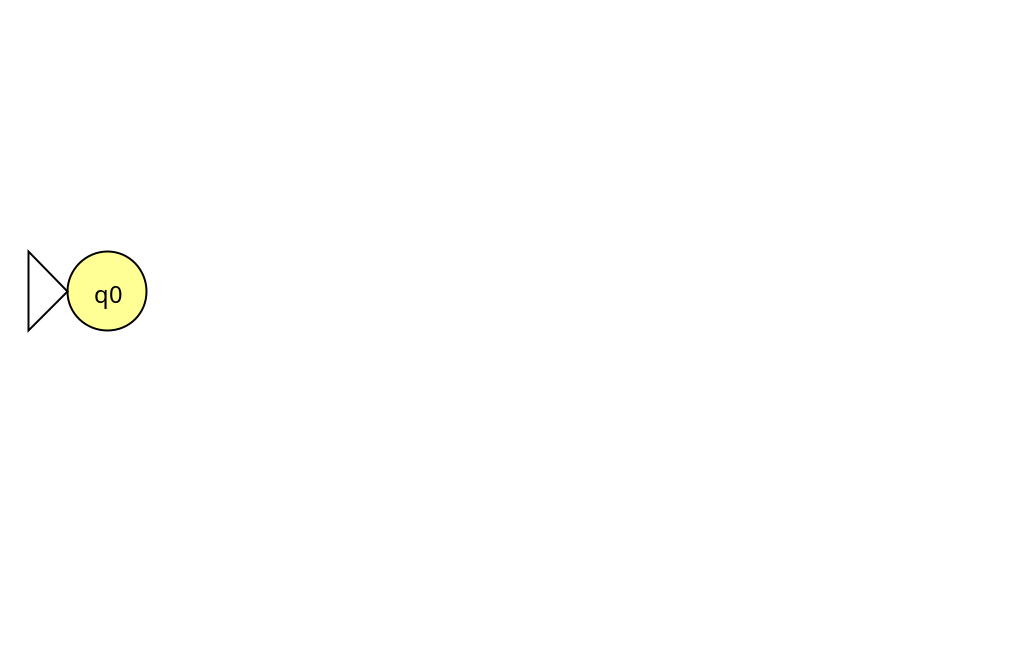
\includegraphics[scale=0.25]{images/mct1ej3_1.png}
    \end{figure}
\end{frame}

%%%%%%%%%%%%%%%%%%%%%%%%%%%%%%%%%%

\begin{frame}{Sección Cuarto de Punto}{Ejercicio 3}
    \textbf{Solución}\\
    \begin{figure}
        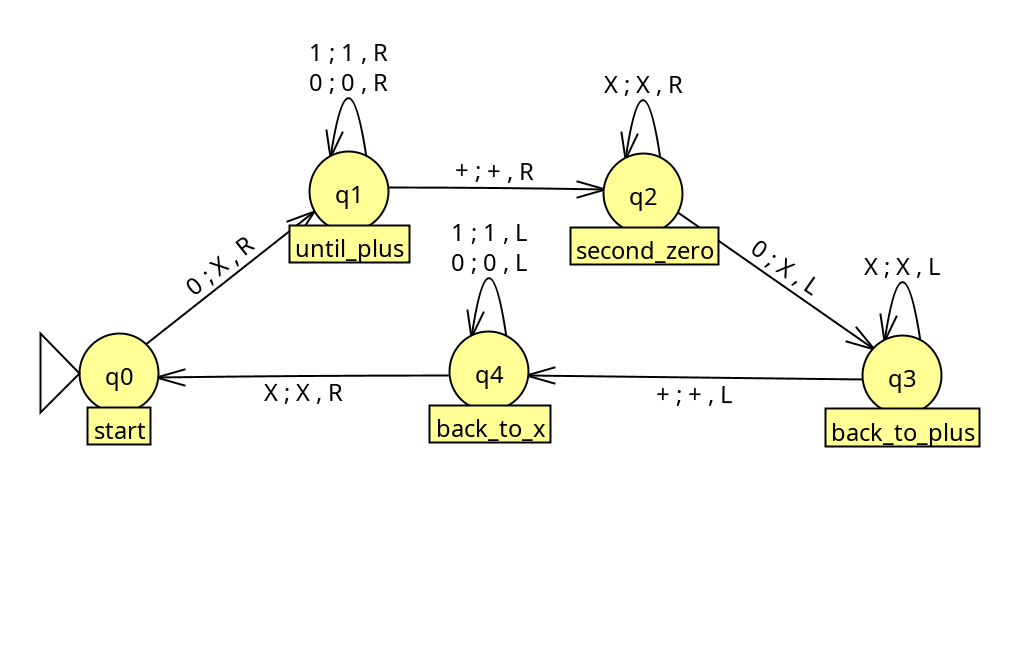
\includegraphics[scale=0.25]{images/mct1ej3_2.png}
    \end{figure}
\end{frame}

%%%%%%%%%%%%%%%%%%%%%%%%%%%%%%%%%%

\begin{frame}{Sección Cuarto de Punto}{Ejercicio 3}
    \textbf{Solución}\\
    \begin{figure}
        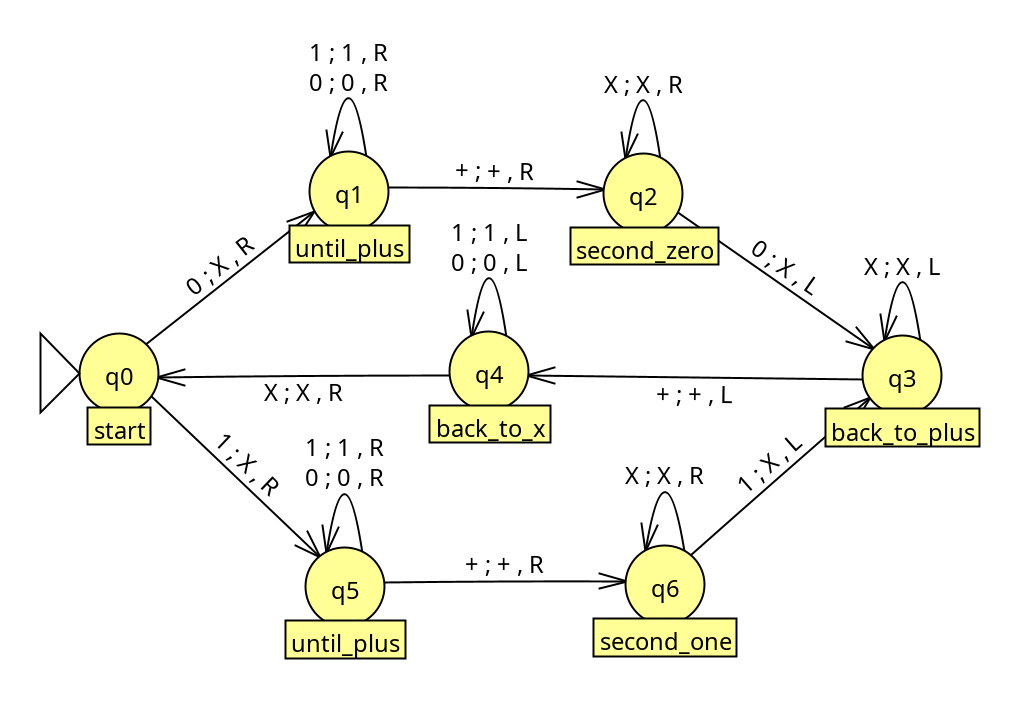
\includegraphics[scale=0.25]{images/mct1ej3_3.png}
    \end{figure}
\end{frame}

%%%%%%%%%%%%%%%%%%%%%%%%%%%%%%%%%%

\begin{frame}{Sección Cuarto de Punto}{Ejercicio 3}
    \textbf{Solución}\\
    \begin{figure}
        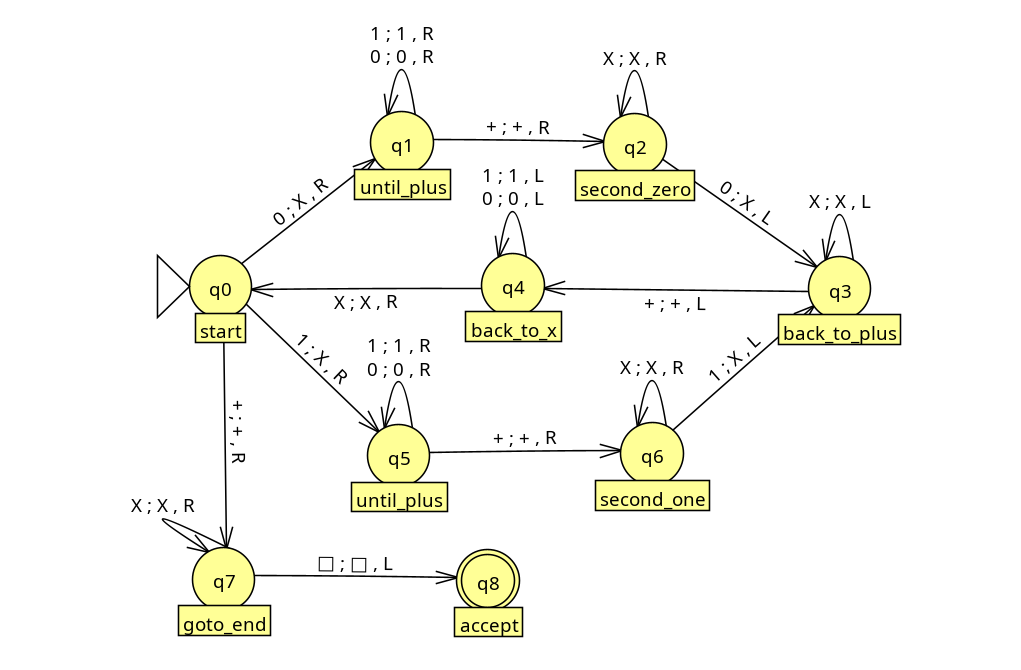
\includegraphics[scale=0.25]{images/mct1ej3_4.png}
    \end{figure}
\end{frame}

%%%%%%%%%%%%%%%%%%%%%%%%%%%%%%%%%%

\begin{frame}{Sección Cuarto de Punto}{Ejercicio 4}
% \vskip -1cm % Para subir (-) o bajar el texto
\textbf{Enunciado}
	\begin{itemize}
        \item Demostrar MT $\equiv$ SMT. Así, describe lo más formalmente posible el mecanismo para, a partir de un MT $M=(Q,\Sigma,\Gamma,\delta,q_0,q_f)$ conseguir la SMT equivalente $M'=(Q',\Sigma,\Gamma,\delta',q_0,q_f)$ y viceveresa.
	\end{itemize}
\end{frame}

%%%%%%%%%%%%%%%%%%%%%%%%%%%%%%%%%%

\begin{frame}{Sección Cuarto de Punto}{Ejercicio 4}
    \textbf{Solución}\\
    MT $\preceq$ SMT\\
    Trivial. Una MT $M=(Q,\Sigma,\Gamma,\delta,q_o,q_f)$ es una SMT sin transiciones con stay.
\end{frame}

%%%%%%%%%%%%%%%%%%%%%%%%%%%%%%%%%%

\begin{frame}{Sección Cuarto de Punto}{Ejercicio 4}
    \textbf{Solución}\\
    SMT $\preceq$ MT\\
    Sea $M=(Q,\Sigma,\Gamma,\delta,q_o,q_f)$ una SMT.\\ 
    Si $M$ no tiene ninguna transición con stay, entonces $M$ es una MT.\\
    Si no, para cada $q_i,q_j \in Q$ y $x,y \in \Gamma$ de forma que existe la transición $\delta(q_i,x)=(q_j,y,S)$ construimos un nuevo estado $q_{i,j,x,y}$.
    Sea $Q'$ el conjunto de estados formado por $Q$ y todos los $q_{i,j,x,y}$.
\end{frame}

%%%%%%%%%%%%%%%%%%%%%%%%%%%%%%%%%%

\begin{frame}{Sección Cuarto de Punto}{Ejercicio 4}
    \textbf{Solución}\\
    Entonces, sobre la quintupla $(Q',\Sigma,\Gamma,q_0,q_f)$ definimos la función $\delta':Q' \times \Gamma \rightarrow Q' \times \Gamma \times \{L,R\}$ definida por:\\
    $\begin{cases}
        \delta'(q_i,x) = (q_j,y,L) & \text{si } \delta(q_i,x) = (q_j,y,L),\\
        \delta'(q_i,x) = (q_j,y,R) & \text{si } \delta(q_i,x) = (q_j,y,R),\\
        \delta'(q_i,x) = (q_{i,j,x,y},y,R) & \text{si } \delta(q_i,x) = (q_j,y,S),\\
        \delta'(q_{i,j,x,y},z) = (q_j,z,L) & \text{si } \delta(q_i,x) = (q_j,y,S) \text{ y } z \in \Gamma\\
    \end{cases}$
\end{frame}

%%%%%%%%%%%%%%%%%%%%%%%%%%%%%%%%%%

\begin{frame}{Sección Cuarto de Punto}{Ejercicio 4}
    \textbf{Solución}\\
    \begin{figure}
        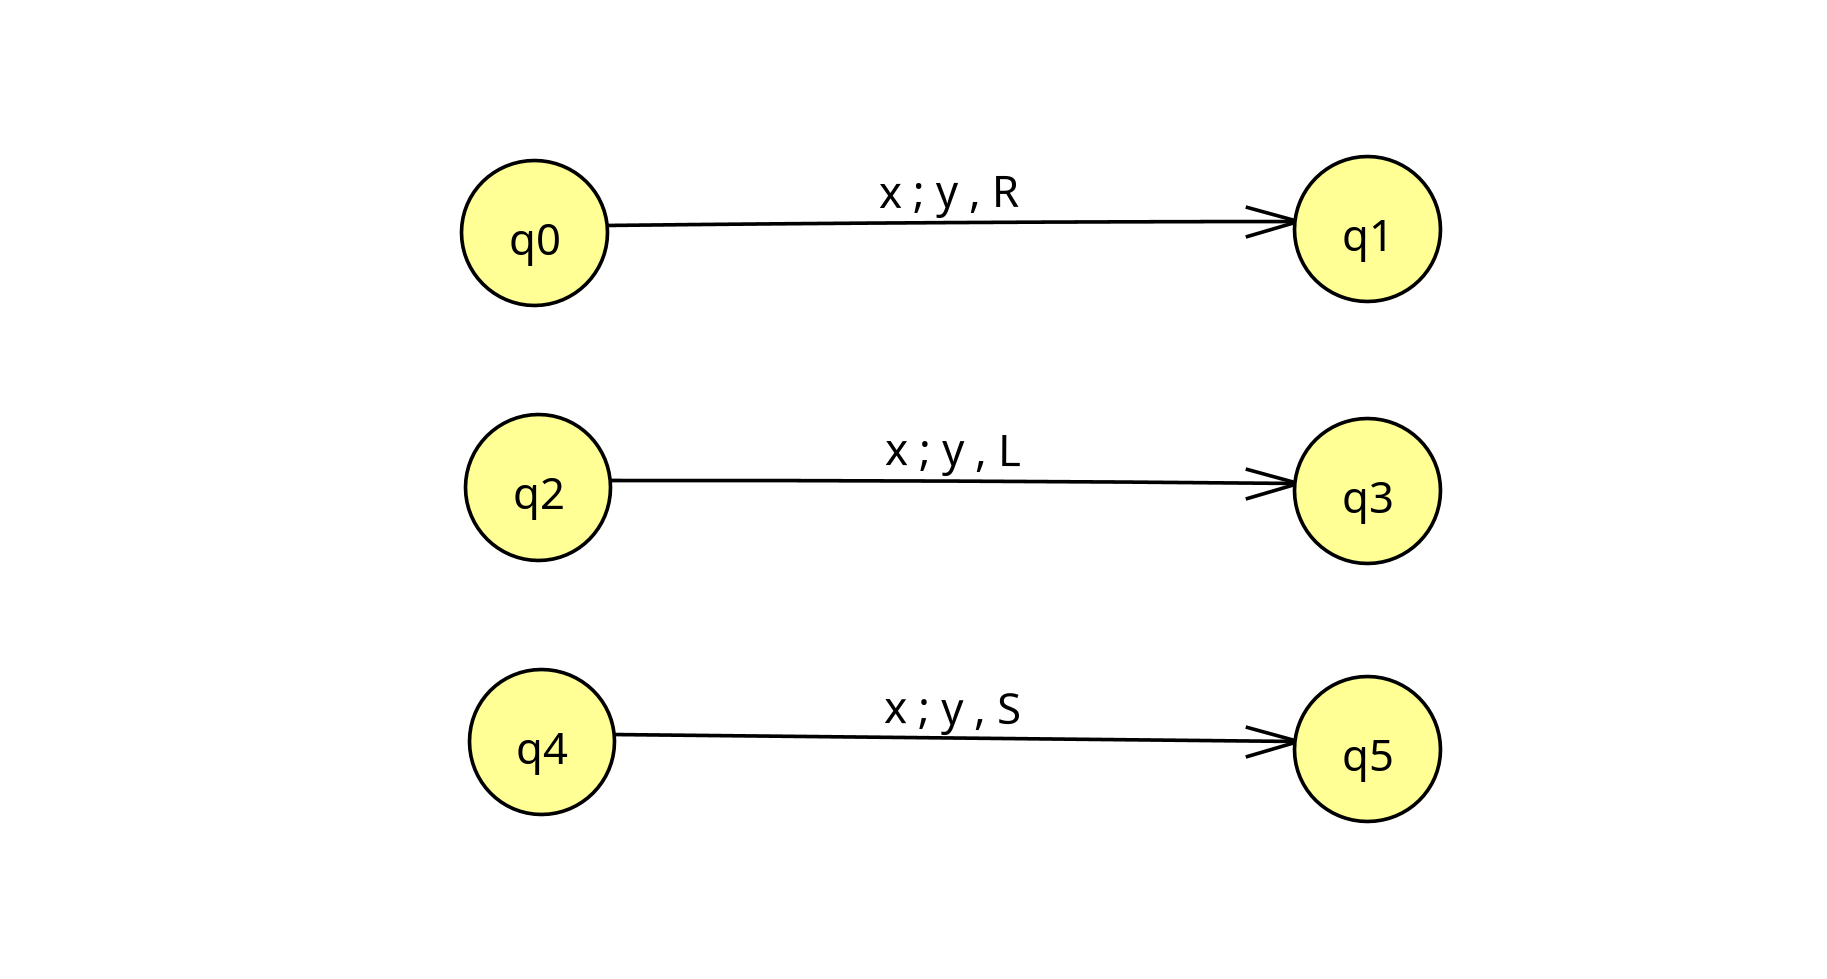
\includegraphics[scale=0.15]{images/mct1ej4_1.png}
    \end{figure}
\end{frame}

%%%%%%%%%%%%%%%%%%%%%%%%%%%%%%%%%%

\begin{frame}{Sección Cuarto de Punto}{Ejercicio 4}
    \textbf{Solución}\\
    \begin{figure}
        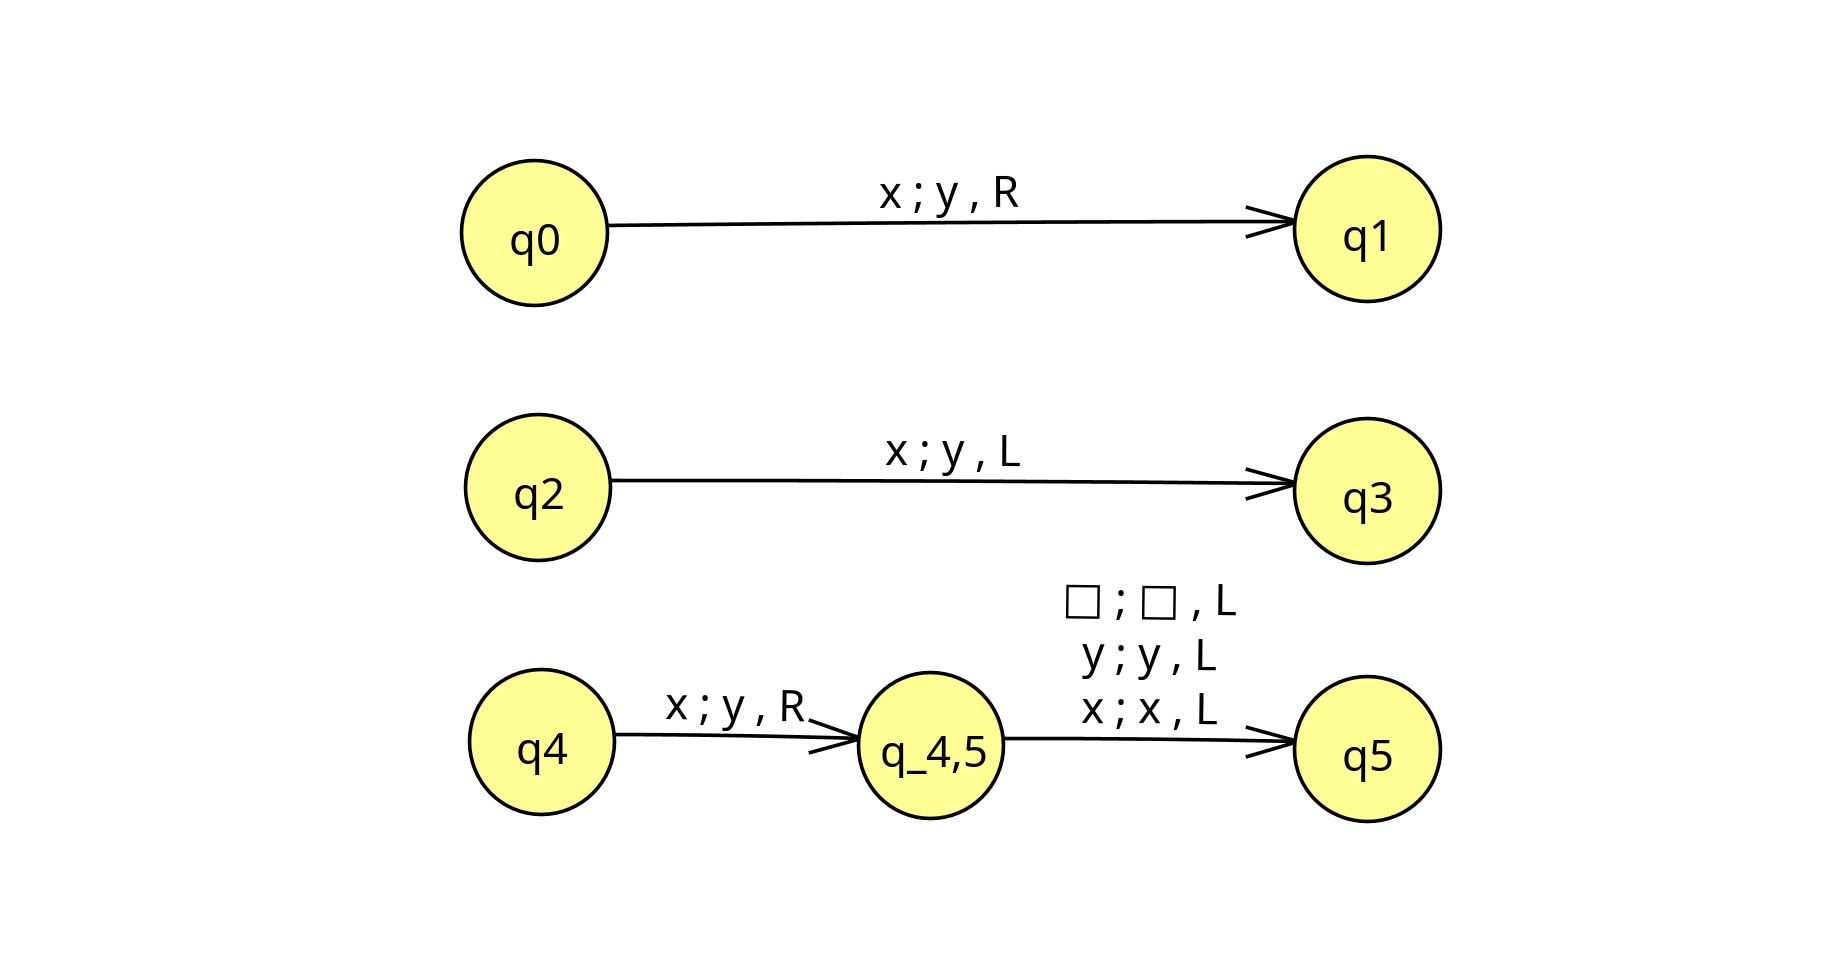
\includegraphics[scale=0.15]{images/mct1ej4_2.png}
    \end{figure}
\end{frame}


%%%%%%%%%%%%%%%%%%%%%%%%%%%%%%%%%%

\begin{frame}{Sección Cuarto de Punto}{Ejercicio 4}
    \textbf{Solución}\\
    \begin{figure}
        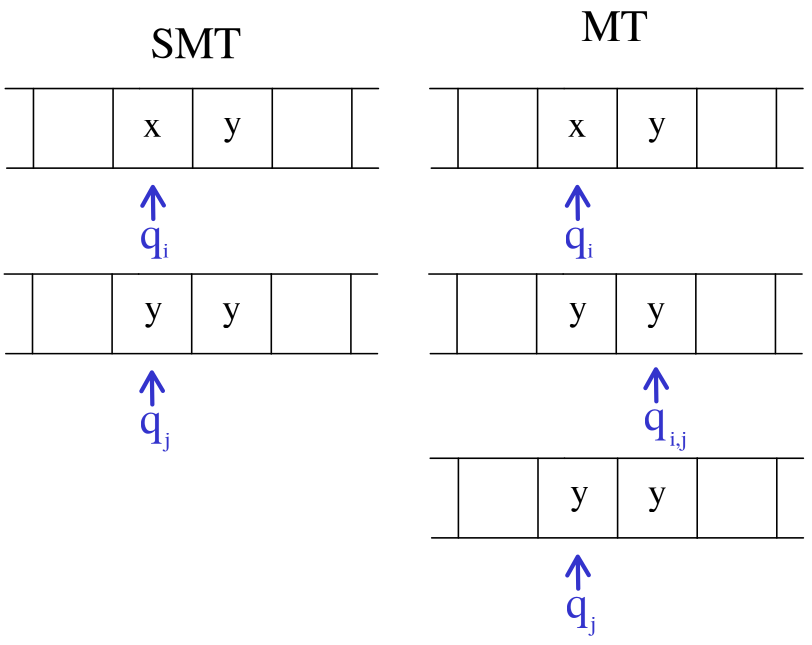
\includegraphics[scale=0.25]{images/mct1ej4_3.png}
    \end{figure}
\end{frame}

%%%%%%%%%%%%%%%%%%%%%%%%%%%%%%%%%%

\begin{frame}{Sección Cuarto de Punto}{Ejercicio 4}
    \textbf{Solución}\\
    Conclusión: apartir de una SMT $M=(Q,\Sigma,\Gamma,\delta,q_o,q_f)$ podemos construir una MT $M'=(Q',\Sigma,\Gamma,\delta',q_o,q_f)$ con un comportamiento análogo.
    Por tanto, SMT $\preceq$ MT, como queríamos demostrar.
\end{frame}

%%%%%%%%%%%%%%%%%%%%%%%%%%%%%%%%%%

\begin{frame}{Sección Cuarto de Punto}{Ejercicio 5}
% \vskip -1cm % Para subir (-) o bajar el texto
\textbf{Enunciado}
	\begin{itemize}
        \item Escribe en pseudocódigo una máquina de Turing para demostrar que el siguiente lenguaje es $\ld$. Acompaña la máquina con la explicación de los aspectos más relevantes. 
        \item[] $$HALT_{Q-steps}^{MT}=\{\langle M \rangle \mbox{ | M es MT y } \exists \omega \mbox{ con la que } M \mbox{ se detiene en }|Q| \mbox{ pasos o menos}  \}$$
    \end{itemize}
\end{frame}

%%%%%%%%%%%%%%%%%%%%%%%%%%%%%%%%%%

\begin{frame}{Sección Cuarto de Punto}{Ejercicio 5}
    \textbf{Solución}\\
    Observación: $\langle M \rangle \in HALT_{Q-steps}^{MT}$ $\Leftrightarrow$ $\exists \omega \text{ con } | \omega | \leq Q$ con la que $M$ se detiene en Q pasos o menos.\\
\end{frame}

%%%%%%%%%%%%%%%%%%%%%%%%%%%%%%%%%%

\begin{frame}{Sección Cuarto de Punto}{Ejercicio 5}
    \textbf{Solución}\\
    \begin{enumerate}
        \item Decodificar la entrada $\langle M \rangle$
        \item $\forall \omega \in \Sigma^* : |\omega| \leq Q$
        \begin{enumerate}
            \item Simular hasta $Q$ pasos de $M(\omega)$
            \item Si $M(\omega)$ acepta o rechaza Entonces ACEPTA
        \end{enumerate}
        \item RECHAZA
    \end{enumerate}
\end{frame}

%%%%%%%%%%%%%%%%%%%%%%%%%%%%%%%%%%

\begin{frame}{Sección Cuarto de Punto}{Ejercicio 6}
% \vskip -1cm % Para subir (-) o bajar el texto
\textbf{Enunciado}
	\begin{itemize}
        \item Escribe una máquina de Turing para demostrar que el siguiente lenguaje es $\lr$. Acompaña la máquina con la explicación de los aspectos más relevantes.\\~\\
    \end{itemize}
    $$ACC_{Q}^{MT}=\{\langle M \rangle \mbox{ | M es una MT y } |L(M)| \geq |Q| \mbox{ siendo Q el conjunto de estados de M}\}$$
\end{frame}

%%%%%%%%%%%%%%%%%%%%%%%%%%%%%%%%%%

\begin{frame}{Sección Cuarto de Punto}{Ejercicio 6}
    % \vskip -1cm % Para subir (-) o bajar el texto
    \textbf{Solución}\\
    Observación: $\langle M \rangle \in ACC_{Q}^{MT} \Leftrightarrow \exists p_M \in \mathbb{N}$ de forma que M acepta al menos $Q$ palabras en menos de $p_M$ pasos.\\~\\
    Dem:\\
    $\boxed{\Rightarrow}$ Si $\langle M \rangle \in ACC_{Q}^{MT}$, existen al menos $Q$ palabras aceptadas por $M$.
    Sean $\omega_1, ..., \omega_Q$ las primeras $Q$ palabras aceptadas por $M$ en un orden lexicográfico y sean $p_1,...,p_Q$ los pasos que requiere $M$ para validar las respectivas entradas.
    Llamamos $p_M = max\{p_i:i=1..Q\}$. $p_M$ cumple la condición buscada.\\
    $\boxed{\Leftarrow} \text{ } M$ acepta al menos $Q$ palabras  $\Rightarrow |L(M)| \geq Q \Rightarrow \langle M \rangle \in ACC_{Q}^{MT}$  
\end{frame}
    

%%%%%%%%%%%%%%%%%%%%%%%%%%%%%%%%%%

\begin{frame}{Sección Cuarto de Punto}{Ejercicio 6}
    \textbf{Solución}\\
    \begin{enumerate}
        \item Decodificar la entrada $\langle M \rangle$
        \item Contar el número de estados y almacenar una constante CONTADOR
        \item $\forall n \in \mathbb{N}$
        \begin{enumerate}
            \item Inicializar un contador CONTADOR2 a cero 
            \item $\forall \omega \in \Sigma^* : |\omega| \leq n$
            \begin{enumerate}
                \item Simular hasta $n$ pasos de $M(\omega)$
                \item Si $M(\omega)$ acepta en n pasos o menos Entonces CONTADOR2++
            \end{enumerate}
            \item Si CONTADOR $\leq$ CONTADOR2 Entonces ACEPTA
        \end{enumerate}
    \end{enumerate}
\end{frame}

%%%%%%%%%%%%%%%%%%%%%%%%%%%%%%%%%%

\begin{frame}{Sección Cuarto de Punto}{Ejercicio 7}
% \vskip -1cm % Para subir (-) o bajar el texto
\textbf{Enunciado}
	\begin{itemize}
        \item Demuestra por contraejemplo que no todo subconjunto de un lenguaje regular es regular y que no todo subconjunto de un lenguaje libre de contexto es libre de contexto.
    \end{itemize}
\end{frame}

%%%%%%%%%%%%%%%%%%%%%%%%%%%%%%%%%%

\begin{frame}{Sección Cuarto de Punto}{Ejercicio 7}
    \textbf{Solución}\\
    Supongamos $\Sigma = \{0,1,2\}$ y tomemos $L = U_\Sigma$ y $L'=\{0^n1^n2^n \mid n \geq 0 \}.$ Entonces $L' \subset L \text{ y } L \in \mathcal{REG} \subset \mathcal{CF}$ pero $L' \notin \mathcal{REG} \text{ y } L' \notin \mathcal{CF}.$
\end{frame}

%%%%%%%%%%%%%%%%%%%%%%%%%%%%%%%%%%

\begin{frame}{Sección Cuarto de Punto}{Ejercicio 7}
    \textbf{Solución}\\
    De hecho, cualquier lenguaje infinito independientemente del alfabeto va a tener subconjuntos incluso altamente indecidibles. Esto se debe a que existe una cantidad numerable de lenguajes Turing-reconocibles, pero el cardinal de las partes de un lenguaje numerable es $2^{\mathcal{N}_0}.$
\end{frame}

%%%%%%%%%%%%%%%%%%%%%%%%%%%%%%%%%%

\begin{frame}{Sección Cuarto de Punto}{Ejercicio 8}
% \vskip -1cm % Para subir (-) o bajar el texto
    \textbf{Enunciado}
    \begin{itemize}
        \item El conjunto $\mt$ de las máquinas de Turing es numerable. La numeración de Gödel es prueba de ello. A partir del lenguaje simple que se ha dado en clase, calcula el número de Gödel de cada una de las instrucciones que componen este fragmento y del fragmento en sí. ¿Es posible que dos fragmentos distintos tengan el mismo número?
        \begin{itemize}
            \item[] $V_1 \coloneqq S(0)$
            \item[] $V_2 \coloneqq S(V_1)$
            \item[] If $S(V_2)!=0$ Then $V_2 \coloneqq0$
            \item[] If $S(V_1)=0$ Then $V_1 \coloneqq S(V_2)$
            \item[] $V_1 \coloneqq S(S(V_2))$
        \end{itemize}
    \end{itemize}
\end{frame}

%%%%%%%%%%%%%%%%%%%%%%%%%%%%%%%%%%

\begin{frame}{Sección Cuarto de Punto}{Ejercicio 8}
    \textbf{Solución}\\
    Recordemos que la numeración de Gödel que se da en las diapositivas de clase es la siguiente:
    \begin{table}[h]
        \centering
        \renewcommand{\arraystretch}{1.2}
        \begin{tabular}{|c|c|}
            \hline
            \textbf{Elemento} & \textbf{Código} \\
            \hline
            0 & 1 \\
            \hline
            \textit{S} & 2 \\
            \hline
            $V_1, V_2, V_3$ & 3,4,5 \\
            \hline
            Asignación & 6 \\
            \hline
            Test = 0 & 7 \\
            \hline
            Test $\neq$ 0 & 8 \\
            \hline
            If Then & 9 \\
            \hline
        \end{tabular}
    \end{table}
\end{frame}

%%%%%%%%%%%%%%%%%%%%%%%%%%%%%%%%%%

\begin{frame}{Sección Cuarto de Punto}{Ejercicio 8}
    \textbf{Solución}\\
    \begin{table}[h]
        \centering
        \renewcommand{\arraystretch}{1.2}
        \begin{tabular}{|c|c|}
            \hline
            \textbf{Elemento} & \textbf{Código} \\
            \hline
            0 & 1 \\
            \hline
            \textit{S} & 2 \\
            \hline
            $V_1, V_2, V_3$ & 3,4,5 \\
            \hline
            Asignación & 6 \\
            \hline
            Test = 0 & 7 \\
            \hline
            Test $\neq$ 0 & 8 \\
            \hline
            If Then & 9 \\
            \hline
        \end{tabular}
    \end{table}
    \begin{itemize}
        \item[1.] $V_1 \coloneqq S(0) \Rightarrow c_1 = 2^3 3^6 5^2 7^1 = 1,020,600$
    \end{itemize}
\end{frame}

%%%%%%%%%%%%%%%%%%%%%%%%%%%%%%%%%%

\begin{frame}{Sección Cuarto de Punto}{Ejercicio 8}
    \textbf{Solución}\\
    \begin{table}[h]
        \centering
        \renewcommand{\arraystretch}{1.2}
        \begin{tabular}{|c|c|}
            \hline
            \textbf{Elemento} & \textbf{Código} \\
            \hline
            0 & 1 \\
            \hline
            \textit{S} & 2 \\
            \hline
            $V_1, V_2, V_3$ & 3,4,5 \\
            \hline
            Asignación & 6 \\
            \hline
            Test = 0 & 7 \\
            \hline
            Test $\neq$ 0 & 8 \\
            \hline
            If Then & 9 \\
            \hline
        \end{tabular}
    \end{table}
    \begin{itemize}
        \item[2.] $V_2 \coloneqq S(V_1) \Rightarrow c_2 = 2^4 3^6 5^2 7^3 = 100,018,800$
    \end{itemize}
\end{frame}

%%%%%%%%%%%%%%%%%%%%%%%%%%%%%%%%%%

\begin{frame}{Sección Cuarto de Punto}{Ejercicio 8}
    \textbf{Solución}\\
    \begin{table}[h]
        \centering
        \renewcommand{\arraystretch}{1.2}
        \begin{tabular}{|c|c|}
            \hline
            \textbf{Elemento} & \textbf{Código} \\
            \hline
            0 & 1 \\
            \hline
            \textit{S} & 2 \\
            \hline
            $V_1, V_2, V_3$ & 3,4,5 \\
            \hline
            Asignación & 6 \\
            \hline
            Test = 0 & 7 \\
            \hline
            Test $\neq$ 0 & 8 \\
            \hline
            If Then & 9 \\
            \hline
        \end{tabular}
    \end{table}
    \begin{itemize}
        \item[3.] If $S(V_2)!=0$ Then $V_2 \coloneqq0 \Rightarrow c_3 = 2^9 3^2 5^4 7^8 11^4 13^6 17^1 = $\\
        $=19,946,035,319,147,107,410,240,000$
    \end{itemize}
\end{frame}

%%%%%%%%%%%%%%%%%%%%%%%%%%%%%%%%%%

\begin{frame}{Sección Cuarto de Punto}{Ejercicio 8}
    \textbf{Solución}\\
    \begin{table}[h]
        \centering
        \renewcommand{\arraystretch}{1.2}
        \begin{tabular}{|c|c|}
            \hline
            \textbf{Elemento} & \textbf{Código} \\
            \hline
            0 & 1 \\
            \hline
            \textit{S} & 2 \\
            \hline
            $V_1, V_2, V_3$ & 3,4,5 \\
            \hline
            Asignación & 6 \\
            \hline
            Test = 0 & 7 \\
            \hline
            Test $\neq$ 0 & 8 \\
            \hline
            If Then & 9 \\
            \hline
        \end{tabular}
    \end{table}
    \begin{itemize}
        \item[4.] If $S(V_1)=0$ Then $V_1 \coloneqq S(V_2) \Rightarrow c_4 = 2^9 3^2 5^3 7^7 11^3 13^6 17^2 19^4 = $\\
        $=114,778,139,142,991,410,757,839,168,000$
    \end{itemize}
\end{frame}

%%%%%%%%%%%%%%%%%%%%%%%%%%%%%%%%%%

\begin{frame}{Sección Cuarto de Punto}{Ejercicio 8}
    \textbf{Solución}\\
    \begin{table}[h]
        \centering
        \renewcommand{\arraystretch}{1.2}
        \begin{tabular}{|c|c|}
            \hline
            \textbf{Elemento} & \textbf{Código} \\
            \hline
            0 & 1 \\
            \hline
            \textit{S} & 2 \\
            \hline
            $V_1, V_2, V_3$ & 3,4,5 \\
            \hline
            Asignación & 6 \\
            \hline
            Test = 0 & 7 \\
            \hline
            Test $\neq$ 0 & 8 \\
            \hline
            If Then & 9 \\
            \hline
        \end{tabular}
    \end{table}
    \begin{itemize}
        \item[5.] $V_1 \coloneqq S(S(V_2)) \Rightarrow c_5 = 2^3 3^6 5^2 7^2 11^4 = 104,958,232,200$
    \end{itemize}
\end{frame}

%%%%%%%%%%%%%%%%%%%%%%%%%%%%%%%%%%

\begin{frame}{Sección Cuarto de Punto}{Ejercicio 8}
    \textbf{Solución}\\
    \begin{itemize}
        \item[] $V_1 \coloneqq S(0)$
        \item[] $V_2 \coloneqq S(V_1)$
        \item[] If $S(V_2)!=0$ Then $V_2 \coloneqq0$
        \item[] If $S(V_1)=0$ Then $V_1 \coloneqq S(V_2)$
        \item[] $V_1 \coloneqq S(S(V_2))$
    \end{itemize}
    $C = 2^{c_1} 3^{c_2} 5^{c_3} 7^{c_4} 11^{c_5} = ...$
\end{frame}

%%%%%%%%%%%%%%%%%%%%%%%%%%%%%%%%%%

\begin{frame}{Sección Cuarto de Punto}{Ejercicio 8}
    \textbf{Solución}\\
    \begin{itemize}
        \item[] $V_1 \coloneqq S(0)$
        \item[] $V_2 \coloneqq S(V_1)$
        \item[] If $S(V_2)!=0$ Then $V_2 \coloneqq0$
        \item[] If $S(V_1)=0$ Then $V_1 \coloneqq S(V_2)$
        \item[] $V_1 \coloneqq S(S(V_2))$
    \end{itemize}
    $C = 2^{c_1} 3^{c_2} 5^{c_3} 7^{c_4} 11^{c_5} = ...$
    $$
        \lfloor log_{10}(C) + 1 \rfloor \approx 9.7 \times 10^{28}
    $$
\end{frame}

%%%%%%%%%%%%%%%%%%%%%%%%%%%%%%%%%%

\begin{frame}{Sección Cuarto de Punto}{Ejercicio 8}
    \textbf{Solución}\\
    ¿Es posible que dos fragmentos distintos tengan el mismo número?
\end{frame}

%%%%%%%%%%%%%%%%%%%%%%%%%%%%%%%%%%

\begin{frame}{Sección Cuarto de Punto}{Ejercicio 8}
    \textbf{Solución}\\
    ¿Es posible que dos fragmentos distintos tengan el mismo número?\\~\\
    Teorema fundamental de la aritmética: el anillo de los números enteros $\mathbb{Z}$ es un dominio de factorización única (DFU).
    Es decir, todo número entero se descompone de forma única como producto de potencias de primos y una unidad. 
\end{frame}

%%%%%%%%%%%%%%%%%%%%%%%%%%%%%%%%%%

\begin{frame}{Sección Cuarto de Punto}{Ejercicio 9}
% \vskip -1cm % Para subir (-) o bajar el texto
    \textbf{Enunciado}
    \begin{itemize}
        \item La Máquina de Turing Universal (también llamada $U$), como todas las MTs tiene un número de Gödel asociado. Aunque el número depende de la codificación elegida, investiga en Internet alguna versión del número de la MT Universal. ¿Cuántos  dígitos tiene? Explica cómo has llegado a la solución.
    \end{itemize}
\end{frame}

%%%%%%%%%%%%%%%%%%%%%%%%%%%%%%%%%%

\begin{frame}{Sección Cuarto de Punto}{Ejercicio 9}
    \textbf{Solución}\\
    ¿Cómo llegamos a la solución?
    \begin{enumerate}
        \item Búsqueda por internet: No encontramos ningún artículo que mencionara el número de Gödel asociado a $U$.
        \item Pregunta a ChatGPT: Respondía que no se suele proporcionar un número específico para la Máquina de Turing Universal.
        \item Consulta bibliografía asignatura: En uno de los libros de la bibliografía complementaria encontramos la respuesta, en concreto en \textit{La nueva mente del emperador} de Roger Penrose.
    \end{enumerate}
\end{frame}

\begin{frame}{Sección Cuarto de Punto}{Ejercicio 9}
    \textbf{Solución}\\
    Este libro tiene un apartado llamado \textit{La Máquina Universal de Turing}, donde se explica cómo se podría construir dicha máquina.
    \vspace{3mm}
    \begin{center}
        \textbf{Idea básica}
    \end{center}
    
    
    Numerar las máquina de Turing. Para ello, se busca codificar las instrucciones en cadenas de 0's y 1's. El autor adopta la siguiente codificación:
    
    \begin{center}
        0 para 0,\hspace{1cm}10 para 1,\hspace{1cm}110 para D,\hspace{1cm}   1110 para I,\hspace{1cm}   11110 para ALTO
    \end{center}

    
\end{frame}

\begin{frame}{Sección Cuarto de Punto}{Ejercicio 9}
    \textbf{Solución}\\
    Por ejemplo, para la máquina de Turing XN+1 (Suma 1 al valor recibido como entrada) se obtiene el siguiente número:
    
    \begin{center}
10101101101001011010100111010010110101111010000111010010101110100010111010100
011010010110110101010101101010101101010100
    \end{center}
    Que en notación decimal estándar se corresponde con:
    \begin{center}
        450 813 704 461 563 958 982 113 775 643 437 908
    \end{center}

    De esta manera, XN+1 es la 450 813 704 461 563 958 982 113 775 643 437 908-ésima máquina de Turing
\end{frame}

\begin{frame}{Sección Cuarto de Punto}{Ejercicio 9}
    \textbf{Solución}\\
    La idea ahora es considerar la acción de la máquina de Turing $T_n$ sobre una cadena finita, que podremos representar en notación binaria (siguiendo nuestro esquema). Sea $m$ su representación binaria. 
    
    \vspace{2mm}
    Suponiendo que la máquina se detiene, obtendremos una respuesta (los dígitos binarios que ha producido la máquina en la cinta). Consideramos nuevamente su representación binaria $p$. 
    \vspace{2mm}
    Podemos expresar la relación entre $n$, $m$ y $p$ de la siguiente forma:
    \begin{center}
        $T_n(m) = p$
    \end{center}
\end{frame}

\begin{frame}{Sección Cuarto de Punto}{Ejercicio 9}
    \textbf{Solución}\\
    Por tanto, dados dos números $n$ y $m$ es posible calcular $p$ viendo el resultado de aplicar la n-ésima máquina de Turing a la entrada $m$.

    \vspace{2mm}
    Se debe codificar ($n$, $m$) en una cinta, utilizando algún separador. En el libro se utiliza 111110 puesto que el sistema de representación de máquinas de Turing que hemos descritos no permite la aparación de cinco 1's consecutivos.

\end{frame}

\begin{frame}{Sección Cuarto de Punto}{Ejercicio 9}
    \textbf{Solución}\\
    $U$ debe leer los dígitos de $n$ (que contiene la descripción de $T_n$ y aplicar las reglas correspondientes a los dígitos de $m$. 
    \vspace{2mm}
    Como bien dice el autor, habrá numerosas idas y vueltas de los números de $n$ a los de $m$ y viceversa. Aún así, se puede dar una lista de instrucciones que permiten realizar este proceso, que nos dan la máquina de Turing universal:

    \begin{center}
        $U(n,m) = T_n(m)$
    \end{center}

    Puesto que U es una máquina de Turing, tiene su número asociado, es decir:
    \begin{center}
        $U = T_u$
    \end{center}
    para cierto $u$. Roger Penrose obtuvo un $u$ de \textbf{1681 cifras}.
    
\end{frame}

%%%%%%%%%%%%%%%%%%%%%%%%%%%%%%%%%%

\begin{frame}{Sección Cuarto de Punto}{Ejercicio 10}
% \vskip -1cm % Para subir (-) o bajar el texto
    \textbf{Enunciado}
    \begin{itemize}
        \item ¿Son decidibles los siguientes lenguajes? ¿Y Turing-reconocibles? Justifica tus respuestas:
        \begin{enumerate}[a)]
            \item  $\{\langle M \rangle \mid \mbox{M es MT y  M es la única MT que acepta } L(M)\}$ 
            \item $\{\langle M \rangle \mid \mbox{M es MT  y  se puede diseñar un programa en Java para reconocer } L(M)\}$
        \end{enumerate}
    \end{itemize}
\end{frame}

%%%%%%%%%%%%%%%%%%%%%%%%%%%%%%%%%%

\begin{frame}{Sección Cuarto de Punto}{Ejercicio 10}
    \textbf{Solución}\\
    \begin{itemize}
        \item[a)] $\mathcal{A} = \{\langle M \rangle \mid \mbox{M es MT y  M es la única MT que acepta } L(M)\}$\\~\\
    \end{itemize}

    Proposición: $\mathcal{A} = \emptyset$\\~\\

    Demostración: supongamos por reducción al absurdo que $\mathcal{A} \neq \emptyset$ y sea $\langle M \rangle \in \mathcal{A}.$
    La máquina de Turing $M$ será de la forma $M=(Q,\Sigma,\Gamma,\delta,q_0,q_f)$. Sea $q' \notin Q$ y sea $M'$ la máquina de Turing $M'=(Q \cup \{q'\},\Sigma,\Gamma,\delta,q_0,q_f)$
    Podemos ver el estado $q'$ como un estado desconectado de los demás. Entonces $L(M) = L(M') \Rightarrow \langle M \rangle \notin \mathcal{A}$.
    Esto es una contradicción pues partíamos de $\langle M \rangle \in \mathcal{A}$   
\end{frame}

%%%%%%%%%%%%%%%%%%%%%%%%%%%%%%%%%%

\begin{frame}{Sección Cuarto de Punto}{Ejercicio 10}
    \textbf{Solución}\\
    \begin{itemize}
        \item[a)] $\mathcal{A} = \{\langle M \rangle \mid \mbox{M es MT y  M es la única MT que acepta } L(M)\}$\\~\\
    \end{itemize}

    Conclusión: el lenguaje es el lenguaje vacío, que es regular y, por tanto, decidible y Turing-reconocible.
\end{frame}

%%%%%%%%%%%%%%%%%%%%%%%%%%%%%%%%%%

\begin{frame}{Sección Cuarto de Punto}{Ejercicio 10}
    \textbf{Solución}\\
    \begin{itemize}
        \item[b)] $\mathcal{B} = \{\langle M \rangle \mid \mbox{M es MT  y  se puede diseñar un programa en Java para reconocer } L(M)\}$\\~\\
    \end{itemize}
    Observación: si M es una MT, $L(M) \in \mathcal{RE}$ y, por ser Java un lenguaje Turing completo, existe un programa en Java que reconoce $L(M)$. Por lo tanto $\mathcal{B} = \{\langle M \rangle \mid \mbox{M es MT}\}$ \\~\\
    
\end{frame}

%%%%%%%%%%%%%%%%%%%%%%%%%%%%%%%%%%

\begin{frame}{Sección Cuarto de Punto}{Ejercicio 10}
    \textbf{Solución}\\
    \begin{itemize}
        \item[b)] $\mathcal{B} = \{\langle M \rangle \mid \mbox{M es MT  y  se puede diseñar un programa en Java para reconocer } L(M)\}$\\~\\
    \end{itemize}
    Observación: si M es una MT, $L(M) \in \mathcal{RE}$ y, por ser Java un lenguaje Turing completo, existe un programa en Java que reconoce $L(M)$. Por lo tanto $\mathcal{B} = \{\langle M \rangle \mid \mbox{M es MT}\}$ \\~\\
    

    Conclusión:\\
    La clase de lenguaje a la que pertenece $\mathcal{B}$ dependerá de la codificación que elijamos para representar una MT. Para codificaciones razonables, el lenguaje será decidible y Turing-reconocible. En particular, si como representación de una MT usamos su número de Gödel, tenemos que $\mathcal{B}$ incluso es regular, ya que $\mathcal{B} = \{\langle M \rangle \mid \mbox{M es MT}\} = L([0-9]^*) \in \mathcal{REG}$
\end{frame}

%%%%%%%%%%%%%%%%%%%%%%%%%%%%%%%%%%

\begin{frame}{Sección Medio Punto}{Ejercicio 11}
% \vskip -1cm % Para subir (-) o bajar el texto
    \textbf{Enunciado}
    \begin{itemize}
        \item Sea $\Sigma=\{0,1,\$\}$. Sea el lenguaje $L=\{x\$x^R\$x \mid x \in \Sigma^*\}$. Demostrar que no es regular: primero explica el lenguaje poniendo algunas palabras ejemplo, luego explica los conceptos teóricos que te van a servir en la demostración, el método de demostración que vas a usar y, finalmente la demostración en si.
    \end{itemize}
\end{frame}

%%%%%%%%%%%%%%%%%%%%%%%%%%%%%%%%%%

\begin{frame}{Sección Medio Punto}{Ejercicio 11}
    \textbf{Solución}\\
    \begin{itemize}
        \item[--] $\$\$$
        \item[--] $0^n \$ 0^n \$ 0^n \text{ donde } n \geq 0$
        \item[--] $ \omega \$ \omega \$ \omega \text{ donde } \omega$ es un palíndromo 
        \item[--] $10\$ \$ \$01 \$ 10\$$  
    \end{itemize}
\end{frame}

%%%%%%%%%%%%%%%%%%%%%%%%%%%%%%%%%%

\begin{frame}{Sección Medio Punto}{Ejercicio 11}
    \textbf{Solución}\\
    Lema del bombeo para lenguajes regulares: si $L \in \mathcal{REG} \text{ entonces } \exists p \in \mathbb{N} \text{ tal que } \forall \omega \in L \text{ con}$
    $|\omega| \geq p$ existe una división $\omega = xyz$ que cumple:
    \begin{itemize}
        \item[a)] $\forall i \geq 0, xy^iz \in L$
        \item[b)] $|y| > 0$
        \item[c)] $|xy| \leq p$  
    \end{itemize}
    El número $p$ se le conoce como longitud de bombeo (pumping length).
\end{frame}

%%%%%%%%%%%%%%%%%%%%%%%%%%%%%%%%%%

\begin{frame}{Sección Medio Punto}{Ejercicio 11}
    \textbf{Solución}\\
    Proposición: el lenguaje $L=\{x\$x^R\$x \mid x \in \Sigma^*\}$ no es regular.\\~\\

    Demostración: supongamos por reducción al absurdo que $L$ es regular y que $p$ es una longitud de bombeo para $L$. 
    Consideremos la palabra $\omega = 0^p\$0^p\$0^p \in L$.\\
    Según el Lema de Bombeo debería existir una división $xyz=\omega$
    que cumpla las tres condiciones. De la segunda ($|y|>0$) y tercera ($|xy| \leq p$) condición se tiene necesariamente $y=0^k, k \in \{1..p\}$ y que $y$ está contenida en la primera ristra de ceros.
    Al bombear $y$ cero veces se obtiene la palabra $xz = 0^{p-k}\$0^p\$0^p \notin L$.\\~\\
    Esto contradice el Lema del Bombeo, por lo que la premisa de suponer que $L$ es regular es incorrecta. 

\end{frame}

%%%%%%%%%%%%%%%%%%%%%%%%%%%%%%%%%%

\begin{frame}{Sección Medio Punto}{Ejercicio 12}
% \vskip -1cm % Para subir (-) o bajar el texto
    \textbf{Enunciado}
    \begin{itemize}
        \item Sea $L= \{ 0^i 1^j 2^k \mid i,j,k \geq0 \mbox{; si } i=1 \mbox{ entonces } j=k \} $. Este lenguaje no es regular. En este caso nos basta con que des una  demostración informal. Pero muestra que, sin embargo,  $L$ sí cumple el Lema del Bombeo para los Lenguajes Regulares.
    \end{itemize}
\end{frame}

%%%%%%%%%%%%%%%%%%%%%%%%%%%%%%%%%%

\begin{frame}{Sección Medio Punto}{Ejercicio 12}
    \textbf{Solución}\\
    Vamos a descomponer $L$ como la unión disjunta de otros tres lenguajes:
    \begin{itemize}
        \item $L_1 = \{ 1^j2^k \mid j,k \geq 0 \}$
        \item $L_2 = \{ 01^j2^j \mid j \geq 0 \}$
        \item $L_3 = \{ 000^i 1^j 2^k \mid i,j,k \geq0\}$
    \end{itemize}
    Es claro que $L = L_1 \cup L_2 \cup L_3$ y que $L_i \cap L_j = \emptyset \text{ } \forall i \neq j$ (solo estamos controlando el número de ceros).
    
    Supongamos por reducción al absurdo que $L \in \mathcal{REG}$. En ese caso, debido a las propiedades de cierre de los lenguajes regurales y dado que $L_1$ y $L_3$ son claramente regulares tendríamos 
    $$L_2 = L \cap \overline{(L_1 \cup L_3)}$$
    Esto es absurdo ya que $L_2$ es un ejemplo clásico de lenguaje no regular (no cumple el lema de bombeo).
    Como consecuencia, $L$ no puede ser regular.
\end{frame}

%%%%%%%%%%%%%%%%%%%%%%%%%%%%%%%%%%

\begin{frame}{Sección Medio Punto}{Ejercicio 12}
    \textbf{Solución}\\
    Proposición: el lenguaje $L= \{ 0^i 1^j 2^k \mid i,j,k \geq0 \mbox{; si } i=1 \mbox{ entonces } j=k \} $ cumple de Bombeo para lenguajes regulares.\\~\\

    Demostración: la longitud de bombeo de este lenguaje es 2 ya que si $\omega \in L$ tiene una longitud mayor o igual que $2$ podemos:
    \begin{itemize}
        \item Si empieza por 1 o 2, bombeamos el primer carácter: \textbf{1}11222
        \item Si empieza por un 0 y el siguiente carácter es distinto a 0, bombeamos el 0: \textbf{0}111222
        \item Si $\omega = 00$, bombeamos el primer 0: \textbf{0}0
        \item Si $\omega>2$, empieza por 00 y le sigue un 1 o un 2, bombeamos 00: \textbf{00}11122
        \item Si $\omega>2$ y empieza por 000, bombeamos el primer 0: \textbf{0}0022
    \end{itemize}
    La longitud de bombeo no puede ser 1, ya que falla el caso $\omega = 00112$.
\end{frame}

%%%%%%%%%%%%%%%%%%%%%%%%%%%%%%%%%%

\begin{frame}{Sección Medio Punto}{Ejercicio 12}
    \textbf{Solución}\\
    Proposición: el lenguaje $L_2 = \{ 01^j2^j \mid j \geq 0 \}$ no cumple el Lema de Bombeo para lenguajes regulares.\\~\\

    Demostración: supongamos que $L_2$ cumple el Lema del Bombeo y sea $p>0$ su longitud de bombeo (descartamos $p=1$ trivialmente). 
    Sea $\omega = 01^p2^p \in L_2$. Si existiera una subdivisión de $\omega = xyz$, tal que $|xy| \leq p$ o bien $y=01^k$ con $0\leq k < p$ (en cuyo caso no se podría bombear con $i \neq 1$ pues solo puede haber un cero en la palabra)
    o bien $y=1^k$ con $0<k\leq p$ (no pudiendo bombear con $i \neq 1$ por mantener la igualdad en con el numero de doses). Se llega entonces a un absurdo y, por tanto, $L_2$ no cumple el Lema de Bombeo.
\end{frame}
    
%%%%%%%%%%%%%%%%%%%%%%%%%%%%%%%%%%

\begin{frame}{Sección Medio Punto}{Ejercicio 13}
% \vskip -1cm % Para subir (-) o bajar el texto
    \textbf{Enunciado}
    \begin{itemize}
        \item Rellena cada casilla de la siguiente tabla con la clase más específica a la que pertenece el lenguaje  $\overline{L_1 \setminus L_2}$ siendo $L_1$ un lenguaje que cumple el supuesto expresado por su fila y $L_2$ siendo un lenguaje que cumple el supuesto dado por su columna. Si algún caso no se puede saber, puedes poner   $"?"$. Justifica cada casilla.\\
    \end{itemize}
\end{frame}

%%%%%%%%%%%%%%%%%%%%%%%%%%%%%%%%%%

\begin{frame}{Sección Medio Punto}{Ejercicio 13}
    \textbf{Solución}\\
    \begin{table}[h]
             \begin{tabular}{|l|l|l|l|}
             \hline
             &&&\\
             &$L_2 \in \mathcal{CF}$ &$ L_2 \in \ld$ & $ L_2 \in \lr$\\
             \hline
             &&&\\
              $ L1 \in \lreg$&(1) $\mathcal{CF}$ &(2) \ld&(3)\lr\\
              \hline
             &&&\\
             $ L1 \subset L$, con $L \in \mathcal{CF}$&(4) $U_\Sigma$&(5) $U_\Sigma$&(6) $U_\Sigma$\\
              \hline
             &&&\\
             $L1 \in CO-\lr $&(7) \lr&(8) \lr&(9) \lr\\
              \hline
             &&&\\
             $L1 \in \lr \cap CO-\lr$&(10) \ld&(11) \ld&(12) \lr\\
              \hline
             &&&\\
             $ L1 \in \lr \setminus CO-\lr$&(13) CO-\lr &(14) CO-\lr&(15) $U_\Sigma$\\
              \hline
             \end{tabular}
        \end{table}
\end{frame}

\begin{frame}{Sección Medio Punto}{Ejercicio 13}
    \textbf{Solución}\\
    Para empezar, aplicaremos las leyes de Morgan al lenguaje $\overline{L_1 \setminus L_2}$:
    
    \begin{center}
        $\overline{L_1 \setminus L_2} = \overline{L_1 \cap \overline{L_2}}= \overline{L_1}\cup L_2 $
    \end{center}

    Esta igualdad se utilizará las siguientes justificaciones:
    
    \begin{enumerate}[(1)]
        \item Como $L_1 \in$ \lreg, sabemos que $\overline{L_1} \in$ \lreg. Al tomar la unión con un lenguaje $\mathcal{CF}$, solo podemos asegurar que sea $\mathcal{CF}$, pues \lreg $\in$ $\mathcal{CF}$ y la unión de lenguajes $\mathcal{CF}$ \space es $\mathcal{CF}$.
        \item Análogo al anterior, aplicado a lenguajes \ld, ya que también cumplen que son cerrados para la unión.
        \item Ídem, los lenguajes \lr \space son también cerrados para la unión.
    \end{enumerate}
\end{frame}

\begin{frame}{Sección Medio Punto}{Ejercicio 13}
    \textbf{Solución}\\
    .
    \begin{enumerate}[label=(\arabic*)]
        \item[(4, 5, 6)] La inclusión no conserva ninguna de las propiedades. Solo podemos decir que estos lenguajes pertencen al conjunto de todos los lenguajes, es decir, $U_\Sigma$
        \item[(7, 8, 9)] Por ser $L_1 \in CO-\lr$, sabemos que $\overline{L_1} \in \lr$, por la propia definición de lenguaje $CO-\lr$. \lr \space es cerrado para la unión, pero no podemos decir nada más acerca de la unión de un lenguaje \lr \space con uno $\mathcal{CF}$ \space o \ld. Por tanto, los tres pertenecen a \lr.
    \end{enumerate}
\end{frame}

\begin{frame}{Sección Medio Punto}{Ejercicio 13}
    \textbf{Solución}\\
    .
    \begin{enumerate}[label=(\arabic*)]
        \item[(10, 11)] Como $L_1 \in$ \lr $\cap CO-$ \lr $\Rightarrow L_1 \in$ \ld, que es cerrado para la unión $\Rightarrow$ Ambos son \ld
        \item[(12)] $L_1\in$ \ld $\subset$ \lr y  \lr \space cerrado para la unión $\Rightarrow$ El lenguaje es \lr
        \item[(13, 14)] $L_1 \in$ \lr $\Rightarrow \overline{L_1} \in CO-$ \lr. Como $\mathcal{CF}$ $\in$ \ld $\subset CO-$ \lr y ser $CO-$ \lr se conserva mediante la unión (Si $L_1$ y $L_2$ son $CO-$ \lr, sus complementarios son \lr. Entonces $\overline{L_1} \cap \overline{L_2} = \overline{L_1 \cup L_2} \in$ \lr por ser \lr cerrado para la intersección. Pero entonces $L_1 \cup L_2 \in CO-$ \lr, como queríamos ver), entonces ambos lenguajes son $CO-$ \lr
        \item[(15)] Este lenguaje es la unión de un lenguaje $CO-$ \lr y otro \lr, por lo que no sabemos nada.
    \end{enumerate}
\end{frame}
%%%%%%%%%%%%%%%%%%%%%%%%%%%%%%%%%%

\begin{frame}{Sección Medio Punto}{Ejercicio 14}
% \vskip -1cm % Para subir (-) o bajar el texto
    \textbf{Enunciado}
    \begin{itemize}
        \item Se tienen las hipótesis de A a E y se tienen las conclusiones de I a V. Se pide conectar cada hipótesis con las conclusiones que se pueden deducir de cada una (pueden ser varias) y dar una breve explicación.
    \end{itemize}
\end{frame}

%%%%%%%%%%%%%%%%%%%%%%%%%%%%%%%%%%

\begin{frame}{Sección Medio Punto}{Ejercicio 14}
% \vskip -1cm % Para subir (-) o bajar el texto
    \textbf{Hipótesis}
    \begin{enumerate}[A.]
        \item $\overline{L} \in CO-\lr$, $X$ es \lr-completo y $X \le_m  L$
        \item El cardinal de $L$ es un número natural
        \item $L \le_m  EQ^{DFA}$  
        \item $EQ^{MT} \le_m L$ 
        \item Existe una MT que acepta las cadenas que son de $L$ y una MT que acepta las cadenas que no son de $L$. 
    \end{enumerate}
\end{frame}

%%%%%%%%%%%%%%%%%%%%%%%%%%%%%%%%%%

\begin{frame}{Sección Medio Punto}{Ejercicio 14}
% \vskip -1cm % Para subir (-) o bajar el texto
    \textbf{Conclusiones}
    \begin{enumerate}[I.]
        \item $L$ es  decidible.
        \item $L$ cumple el Lema de Bombeo para los Lenguajes  libres de contexto.
        \item se puede construir una MT que rechace las cadenas que son de $L$ y que acepte las cadenas que no son de $L$.
        \item $L$ no es recursivamente enumerable.
        \item $L$ es \lr-completo. 
    \end{enumerate}
\end{frame}

%%%%%%%%%%%%%%%%%%%%%%%%%%%%%%%%%%



\begin{frame}{Sección Medio Punto}{Ejercicio 14}
    \textbf{Solución}\\
     \begin{center}
        A. $\overline{L} \in CO-$ \lr, $X$ es \lr-completo y $X \le_m  L$
    \end{center}
    Como $\overline{L} \in CO-$ \lr $\Rightarrow L\in$ \lr \\ 
    Por ser X \lr-completo y $X \leq_m L$, sabemos que L es \lr-completo. Por tanto:\\
    \begin{center}
        $A. \Rightarrow V.$
    \end{center}
    No se puede deducir ninguna otra de las conclusiones a partir de A.
\end{frame}

\begin{frame}{Sección Medio Punto}{Ejercicio 14}
    \textbf{Solución}\\
     \begin{center}
        B. El cardinal de $L$ es un número natural
    \end{center}
    De la afirmación B deducimos que $L \in$ \lreg. Por tanto, podemos deducir:
    \begin{enumerate}[I.]
        \item L es dedicible: \lreg $\subset$ \ld $\Rightarrow L \in$ \ld
        \item \lreg $\subset$ \lcf $\Rightarrow L \in$ \lcf $\Rightarrow$ Cumple el Lema de Bombeo para los Lenguajes libres de contexto.
        \item Por ser L decidible, podemos construir una máquina de Turing que rechace las cadenas que son de L y que acepte las que no son de L.
    \end{enumerate}
    %\vspace{3}
    %No se puede deducir ninguna otra de las conclusiones a partir de B.
\end{frame}

\begin{frame}{Sección Medio Punto}{Ejercicio 14}
    \textbf{Solución}\\
     \begin{center}
        C. $L \le_m  EQ^{DFA}$  
    \end{center}
    $EQ^{DFA} = \{\langle A_1, A_2\rangle \space \mid \space A_1 \text{ y } A_2 \text{ son DFA tal que } L(A_1) = L(A_2)\}$  que hemos visto en clase que es decidible.
    \vspace{3mm}
    Aplicando el 1er Teorema de Reducibilidad, sabemos que $L\in$ \ld, es decir: 
    \begin{center}
        $C. \Rightarrow I.$
    \end{center}
    Por ser L decidible, podemos construir la máquina de Turing de III, por tanto: 
    \begin{center}
        $C. \Rightarrow III.$
    \end{center}
    No se puede deducir ninguna otra de las conclusiones a partir de C.
     
\end{frame}

\begin{frame}{Sección Medio Punto}{Ejercicio 14}
    \textbf{Solución}\\
     \begin{center}
        D. $EQ^{MT} \le_m L$   
    \end{center}
    $EQ^{MT} = \{\langle M_1, M_2\rangle \space | \space M_1 \text{ y } M_2 \text{ son MT tal que } L(M_1) = L(M_2)\}$. Veamos que este lenguaje no es \lr. Una vez tengamos esto, por el 2ndo Teorema de Reducibilidad tendremos que $L\notin \lr$, es decir:
    \begin{center}
        $D. \Rightarrow IV.$
    \end{center}
\end{frame}


\begin{frame}{Sección Medio Punto}{Ejercicio 14}
    \textbf{Solución}\\
     \begin{center}
        \textbf{Proposición.} $EQ^{MT} \notin$ \lr
    \end{center}
    Supongamos que $EQ^{MT}\in$ \lr. Entonces se puede construir la siguiente mapping-reducción desde $EMPTY^{MT}$:
    
    \vspace{3mm}
    Sea $M_{\emptyset}$ la máquina de Turing que acepta el lenguaje vacío. Dada una MT $M \in EMPTY^{MT}$, tenemos que $\langle M, M_{\emptyset}\rangle \in EQ^{MT}$. Por tanto, $EMPTY^{MT} \leq_{m} EQ^{MT}$. Pero esto implicaría que $EMPTY^{MT}$ es $\mathcal{RE} \space$ por el 2ndo Teorema de Reducibilidad. CONTRADICCIÓN.
    
    \vspace{3mm}
    Queda demostrado por reducción al absurdo que $EQ^{MT} \notin$ \lr\\
    
    \vspace{3mm}
    No se puede deducir ninguna otra de las conclusiones a partir de D.
    
\end{frame}

\begin{frame}{Sección Medio Punto}{Ejercicio 14}
    \textbf{Solución}\\
     \begin{center}
        E. Existe una MT que acepta las cadenas que son de $L$ y una MT que acepta las cadenas que no son de $L$.   
    \end{center}
    Utilizando estas dos MTs ($M_1$ y $M_2$) se puede construir una MT M' que decide L:
    Ante una entrada $\omega$, M' actúa así:
    \begin{enumerate}[1.] 
        \item Ejecuta paralelamente $M_1$ y $M_2$ con $\omega$ (ejecutar pasos alternadamente). 
        \item   Si $M_1$ ACEPTA, M' ACEPTA.\\
                Si $M_2$ ACEPTA, M' RECHAZA.
    \end{enumerate}
        
    \vspace{3mm}
    Sabemos que es proceso terminará en tiempo finito, pues o bien $\omega \in L$ o $w \notin L$.
    Por tanto sabemos que L es decidible, es decir:
    \begin{center}
        $E. \Rightarrow I.$
    \end{center}
\end{frame}

\begin{frame}{Sección Medio Punto}{Ejercicio 14}
    \textbf{Solución}\\
     \begin{center}
        E. Existe una MT que acepta las cadenas que son de $L$ y una MT que acepta las cadenas que no son de $L$.   
    \end{center}
    Obviamente, también se cumple: 
    \begin{center}
        $E. \Rightarrow III.$
    \end{center}
    Construimos la máquina M' que nos piden en III:\\
    Ante una entrada $\omega$, M' actúa así:
    \begin{enumerate}[1.] 
        \item Ejecuta paralelamente $M_1$ y $M_2$ con $\omega$. 
        \item   Si $M_1$ ACEPTA, M' RECHAZA.\\
                Si $M_2$ ACEPTA, M' ACEPTA.
    \end{enumerate}

    \vspace{3mm}
    Igual que antes, sabemos que terminará en tiempo finito.
    
\end{frame}
%%%%%%%%%%%%%%%%%%%%%%%%%%%%%%%%%%

\begin{frame}{Sección Medio Punto}{Ejercicio 15}
% \vskip -1cm % Para subir (-) o bajar el texto
    \textbf{Enunciado}
    \begin{itemize}
        \item Demuestra la indecibilidad de K y la indecibilidad del Problema de la Parada usando descripciones gráficas de las MTs.
    \end{itemize}
\end{frame}

%%%%%%%%%%%%%%%%%%%%%%%%%%%%%%%%%%

\begin{frame}{Sección Medio Punto}{Ejercicio 15}
    \textbf{Solución}\\
    $$
    K=Acc^{MT}=\{ \langle M, \omega \rangle \mid M \text{ acepta } \omega \} \in \mathcal{DEC} \text{?}
    $$
    \begin{figure}
        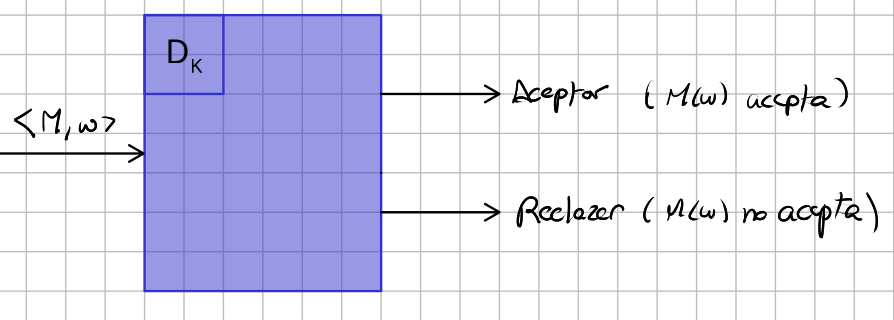
\includegraphics[scale=0.40]{images/DK.png}
    \end{figure}
\end{frame}

%%%%%%%%%%%%%%%%%%%%%%%%%%%%%%%%%%

\begin{frame}{Sección Medio Punto}{Ejercicio 15}
    \textbf{Solución}\\
    $$
    K \in \mathcal{DEC} \Rightarrow \overline{K} \in \mathcal{DEC}
    $$
    \begin{figure}
        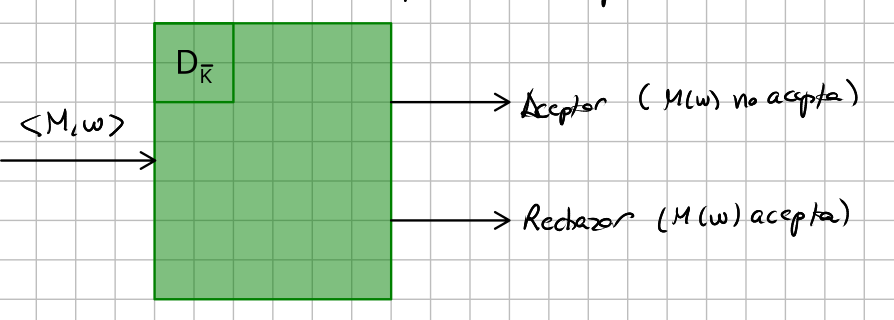
\includegraphics[scale=0.40]{images/DK2.png}
    \end{figure}
\end{frame}

%%%%%%%%%%%%%%%%%%%%%%%%%%%%%%%%%%

\begin{frame}{Sección Medio Punto}{Ejercicio 15}
    \textbf{Solución}\\
    $$
    L = \{ \langle M \rangle \mid \langle M, \langle M \rangle \rangle \in \overline{K} \} 
    $$
    \begin{figure}
        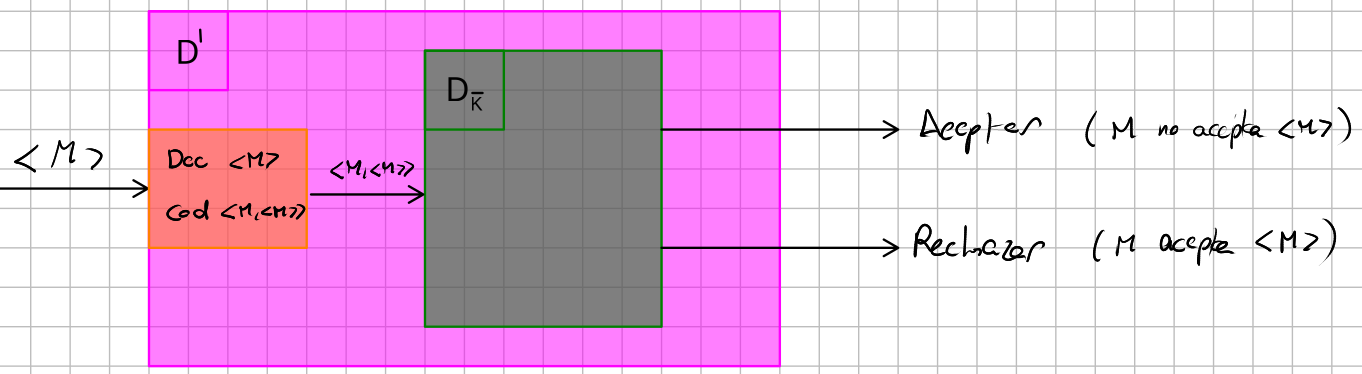
\includegraphics[scale=0.29]{images/D1.png}
    \end{figure}
\end{frame}

%%%%%%%%%%%%%%%%%%%%%%%%%%%%%%%%%%

\begin{frame}{Sección Medio Punto}{Ejercicio 15}
    \textbf{Solución}\\
    \begin{center}
        ¿Cómo se comporta $D'$ con su propia codificación?
    \end{center}
    \begin{figure}
        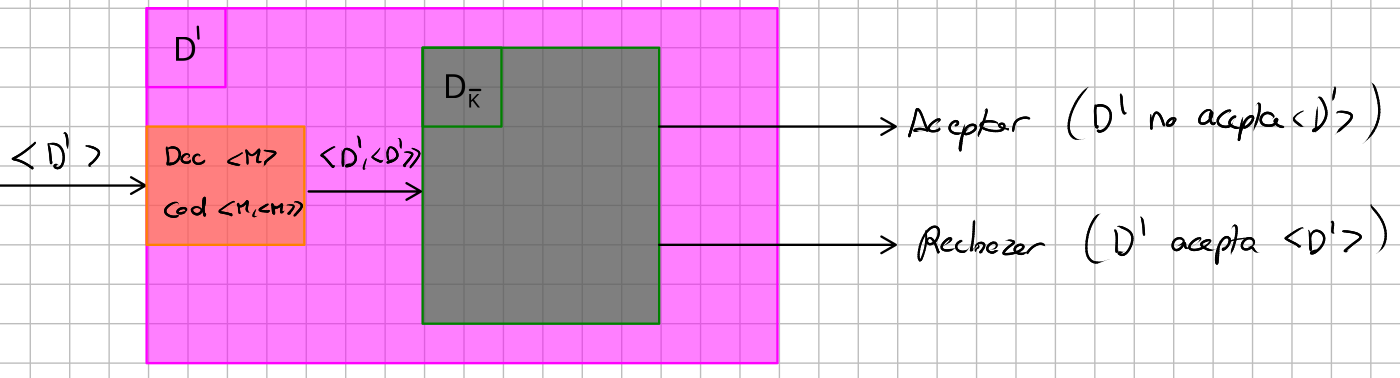
\includegraphics[scale=0.28]{images/D2.png}
    \end{figure}
\end{frame}

%%%%%%%%%%%%%%%%%%%%%%%%%%%%%%%%%%

\begin{frame}{Sección Tres Cuartos de Punto}{Ejercicio 16}
% \vskip -1cm % Para subir (-) o bajar el texto
    \textbf{Enunciado}
    \begin{itemize}
        \item Demuestra que la operación de clausura es cerrada en $\lr$. Puedes usar una MT de alto nivel, pero da una breve explicación y detalla los aspectos claves de su funcionamiento.
    \end{itemize}
\end{frame}

%%%%%%%%%%%%%%%%%%%%%%%%%%%%%%%%%%

\begin{frame}{Sección Tres Cuartos de Punto}{Ejercicio 16}
    \textbf{Solución}\\
    Observación 1: sea $L$ un lenguaje Turing-reconocible no vacío. 
    Entonces $\omega \in L^*$ si y solo si existe un número natural $k \in \mathbb{N}$ y una subdivisión $\omega = \omega_1...\omega_k$ donde $\omega_i \in L \text{ } \forall i = 1..k$\\~\\

    Observación 2: sea $\omega$ una palabra de longitud $|\omega|=n$ y sea $1 \leq k \leq n$.
    Entonces existen ${n-1}\choose{k-1}$ subdivisiones disintas de $\omega$ en $k$ subpalabras.
\end{frame}

%%%%%%%%%%%%%%%%%%%%%%%%%%%%%%%%%%

\begin{frame}{Sección Tres Cuartos de Punto}{Ejercicio 16}
    \textbf{Solución}\\
    Observación 1: sea $L$ un lenguaje Turing-reconocible no vacío. 
    Entonces $\omega \in L^*$ si y solo si existe un número natural $k \in \mathbb{N}$ y una subdivisión $(\omega_1,...,\omega_k)$ de $\omega$ donde $\omega_i \in L \text{ } \forall i = 1..k$\\~\\

    Observación 2: sea $\omega$ una palabra de longitud $|\omega|=n$ y sea $1 \leq k \leq n$.
    Entonces existen ${n-1}\choose{k-1}$ subdivisiones disintas de $\omega$ en $k$ subpalabras.\\~\\

    Esto se debe a que para subdividir $\omega$ en $k$ trozos hay que elegir $(k-1)$ de los $(n-1)$ "cortes" posibles.
\end{frame}

%%%%%%%%%%%%%%%%%%%%%%%%%%%%%%%%%%

\begin{frame}{Sección Tres Cuartos de Punto}{Ejercicio 16}
    \textbf{Solución}\\
    Teorema: $\mathcal{RE}$ es cerrado por clausuras.\\~\\
    Notación: Llamaremos $S_{\omega, k}$ al conjunto de subdivisiones de $\omega$ en $k$ trozos.\\~\\ 
    Demostración: sea $L$ un lenguaje Turing-reconocible reconocido por la máquina $M$. Si $L$ es vacío, $M$ reconoce $L^*=L=\emptyset$. Si no, partir de $M$ construimos la máquina $M^*$ que ante una entrada $\omega$:
    \begin{enumerate}
        \item Si $\omega = \epsilon$ Entonces ACCEPT 
        \item Recorre $\omega$ para contar el número de letras que la forman y almacenar el resultado en N
        \item $\forall i \in \mathbb{N}$
        \begin{enumerate}
            \item $\forall k \in {1,...,N}$
            \begin{enumerate}
                \item $\forall (\omega_1,...,\omega_k) \in S_{\omega, k}$ simular hasta $i$ pasos de $M(\omega_j)$ $\forall j=1..k$
                \item Si $M(\omega_j)$ acepta $\forall j=1..k$ Entonces ACCEPT
            \end{enumerate}
        \end{enumerate}
    \end{enumerate}
\end{frame}

%%%%%%%%%%%%%%%%%%%%%%%%%%%%%%%%%%

\begin{frame}{Sección Tres Cuartos de Punto}{Ejercicio 17}
% \vskip -1cm % Para subir (-) o bajar el texto
    \textbf{Enunciado}
    \begin{itemize}
        \item Justifica la verdad o falsedad de los siguientes enunciados:
        \begin{enumerate}[a)]
            \item Sea $L_2 \in \lr$ y sea $L_1$ tal que $L_1 \subseteq L_2$. Entonces, si $\exists$ un autómata con pila $A$ tal que $L(A)=L_2$ entonces $L_1$ cumple el Lema de Bombeo para los Lenguajes Libres de Contexto. 
            \item Sea $L_2 \in \lr$ y sea $L_1$ tal que $L_1 \subseteq L_2$. Entonces, si no  existe una máquina de Turing con  STAY para decidir $L_1$ entonces no existe una máquina de Turing determinista de 2 cintas para decidir $L_2$.
            \item Sea $L_2 \in \lr$ y sea $L_1$ tal que $L_1 \subseteq L_2$. Entonces, si $L_2 \setminus L_1=\{\lambda\}$ se cumple que si $L_1 \in \ld$ entonces $L_2 \in \ld$ .
            \item ...
        \end{enumerate}
    \end{itemize}
\end{frame}

%%%%%%%%%%%%%%%%%%%%%%%%%%%%%%%%%%

\begin{frame}{Sección Tres Cuartos de Punto}{Ejercicio 17}
    \textbf{a) Sea $L_2 \in \lr$ y sea $L_1$ tal que $L_1 \subseteq L_2$. Entonces, si $\exists$ un autómata con pila $A$ tal que $L(A)=L_2$ entonces $L_1$ cumple el Lema de Bombeo para los Lenguajes Libres de Contexto.}\\~\\
    Sea $L_2$ el lenguaje universal para el alfabeto $\{a,b,c\}$ y sea $L_1=\{a^n b^n c^n \mid n \geq 1\}$.
    Entonces $L_2 \in \mathcal{RE}, L_1 \subseteq L_2$ y existe un autómata con pila que decide $L_2$ pues el lenguaje universal es regular (en particular $L_2 \in \mathcal{CF}$).
    No obstante, $L_1$ no cumple el Lema de Bombeo para los Lenguajes Libres de Contexto.\\~\\
    \textbf{La afirmación es falsa.}
\end{frame}

%%%%%%%%%%%%%%%%%%%%%%%%%%%%%%%%%%

\begin{frame}{Sección Tres Cuartos de Punto}{Ejercicio 17}
    \textbf{b) Sea $L_2 \in \lr$ y sea $L_1$ tal que $L_1 \subseteq L_2$. Entonces, si no  existe una máquina de Turing con  STAY para decidir $L_1$ entonces no existe una máquina de Turing determinista de 2 cintas para decidir $L_2$.}\\~\\

    Sea $L_2$ e lenguaje universal del alfabeto binario y sea $L_1=\{ \langle M \rangle \mid \langle M \rangle$ es el código de Gödel de una máquina de Turing que acepta el lenguaje vacío$\}$.
    Entonces $L_2 \in \mathcal{RE}, L_1 \subset L_2$ y no existe una máquina de Turing con STAY para decidir $L_1$ ya que $L_1$ es indecidible pero si existe una máquina de Turing determinista de 2 cintas para decidir $L_2$ ya que $L_2$ es regular.\\~\\

    \textbf{La afirmación es falsa.}
\end{frame}

%%%%%%%%%%%%%%%%%%%%%%%%%%%%%%%%%%

\begin{frame}{Sección Tres Cuartos de Punto}{Ejercicio 17}
    \textbf{c) Sea $L_2 \in \lr$ y sea $L_1$ tal que $L_1 \subseteq L_2$. Entonces, si $L_2 \setminus L_1=\{\lambda\}$ se cumple que si $L_1 \in \ld$ entonces $L_2 \in \ld$.}\\~\\

    De $L_1 \subseteq L_2$ y $L_2 \setminus L_1 = \{\lambda\}$ tenemos necesariamente $L_2 = L_1 \dot{\cup} \{\lambda\}$.
    De la propiedad de cierre de los lenguajes decidibles bajo la unión $L_1 \in \mathcal{DEC}$ y $\{\lambda\} \in \mathcal{DEC}$ $\Rightarrow L_2 = L_1 \cup \{\lambda\} \in \mathcal{DEC}.$\\~\\

    \textbf{La afirmación es cierta.}

\end{frame}

%%%%%%%%%%%%%%%%%%%%%%%%%%%%%%%%%%

\begin{frame}{Sección Tres Cuartos de Punto}{Ejercicio 17}
    \textbf{d) Si $HALT^{MT} \le_m L$ entonces existe una MT  que acepte las cadenas de $L$ y rechace las cadenas que no son de $L$.}\\~\\    

    Supongamos por reducción al absurdo que existe un decisor $D_L$ para $L$ y que $HALT^{MT}$ se mapping-reduce a $L$ con la función $f$.
    Sea $D_H$ la máquina de Turing que ante una entrada $\langle M,\omega \rangle$:
    \begin{enumerate}[1.]
        \item Aplica $f$ a la entrada $\langle M,\omega \rangle$
        \item Ejecuta $D_L(f(\langle M,\omega \rangle))$
        \item Si $D_L$ acepta Entonces ACCEPTA
        \item Sino RECHAZA
    \end{enumerate}

    Como $f$ es una mapping-reducción y $D_L$ es un decisor, $D_H$ es un decisor para $HALT^{MT}$, lo que es absurdo ya que sabemos que $HALT^{MT}$ no es decidible.
    Por tanto, $D_L$ no puede existir.\\~\\

    \textbf{La afirmación es falsa.}
\end{frame}

%%%%%%%%%%%%%%%%%%%%%%%%%%%%%%%%%%

\begin{frame}{Sección Tres Cuartos de Punto}{Ejercicio 17}
    \textbf{e) El lenguaje $L_{exquisito}$, formado por aquellas MTs que aceptan menos cadenas de las que no aceptan, es indecidible. (además, descríbelo como los lenguajes de clase).}\\
    El cardinal de un lenguaje para un alfabeto finito está acotado por $\mathcal{N}_0$. Como consecuencia, $\langle M \rangle \in L_{exquisito} \Leftrightarrow |L(M)|<\mathcal{N}_0$.
    Así pues, podemos describir el lenguaje como: 
    \begin{center}
        $L_{exquisito}=\{\langle M \rangle \mid |L(M)|< \mathcal{N}_0\}$
    \end{center}
    Aplicando el Teorema de Rice, $L_{exquisito}$ no es decidible, pues tener un cardinal finito no es una propiedad trivial de los lenguajes.\\~\\

    \textbf{La afirmación es verdadera.}
    
\end{frame}

%%%%%%%%%%%%%%%%%%%%%%%%%%%%%%%%%%

\begin{frame}{Sección Tres Cuartos de Punto}{Ejercicio 17}
    \textbf{f) El lenguaje $$L_{not_{murciano}}=\{\langle M \rangle \mid \mbox{M es MT  tal que } |w|\neq |pijo|,  \forall \omega \in L(M) \}$$  no es decidible según el Teorema de Rice}\\~\\
    
    Podemos reescribir la definición del lenguaje de forma que quede más clara la aplicación del Teorema de Rice:
    \begin{center}
        $L_{not_{murciano}}=\{\langle M \rangle \mid M \text{es MT tal que } L(M) \text{ no contiene ninguna palabra de longitud 4}\}$
    \end{center}
    Como contener o no contener palabras de cierta longitud no es una propiedad trivial de los lenguajes, el lenguaje no es decidible.\\~\\

    \textbf{La afirmación es verdadera.}
\end{frame}

%%%%%%%%%%%%%%%%%%%%%%%%%%%%%%%%%%

\begin{frame}{Sección Tres Cuartos de Punto}{Ejercicio 17}
    \textbf{g) Si $L\le_m  Acc^{PDA}$ entonces existe una MT de 2 cintas que decide $L$. }\\~\\
    Es una aplicación directa del \textbf{Primer Teorema de Reducibilidad}. Sabemos que $Acc^{PDA}$ es un lenguaje decidible.
    Como $L$ se mapping-reduce en $Acc^{PDA}$, $L$ también es decidible y existe una MT de 2 cintas que lo decide.\\~\\

    \textbf{La afirmación es verdadera}
\end{frame}

%%%%%%%%%%%%%%%%%%%%%%%%%%%%%%%%%%

\begin{frame}{Sección Tres Cuartos de Punto}{Ejercicio 17}
    \textbf{h) Dada  una propiedad trivial $PT$ de los lenguajes \lr \space y $L_{PT}=\{\langle M \rangle \mid \hbox{ M es una MT cuyo lenguaje no cumple } PT\}$, $L_{PT}$ es decidible y la MT que lo decide es una que siempre rechaza su entrada.}\\~\\
   
    Sea $PT$ la propiedad $ \notin \mathcal{RE}$ entonces $L_{PT} = \{\langle M \rangle \mid M \text{ es una MT cuyo lenguaje no cumple } L(M) \notin \mathcal{RE}\}$, es decir, $L_{PT} = \{\langle M \rangle \mid M \text{ es una MT cuyo lenguaje cumple } L(M) \in \mathcal{RE}\} = {\langle M \rangle \mid M es una MT}$
    Así pues, $L_{PT}$ es decidible, pero la MT que lo decide siempre acepta su entrada.\\~\\

    \textbf{La afirmación es falsa.}
\end{frame}

%%%%%%%%%%%%%%%%%%%%%%%%%%%%%%%%%%

\begin{frame}{Sección Tres Cuartos de Punto}{Ejercicio 18}
% \vskip -1cm % Para subir (-) o bajar el texto
    \textbf{Enunciado}
    \begin{itemize}
        \item ¿Son decidibles los siguientes lenguajes? ¿Y Turing-reconocibles? Justifica tus respuestas:
        \begin{enumerate}[a)]
            \item $\{\langle M \rangle \mid \hbox{ M es una MT con } |L(M)| \geq 100\}$ (por mapping-reducción desde $HALT^{MT}$)
            \item $\{\langle M \rangle \mid \hbox{ M es una MT con lenguaje finito}  \}$ (por mapping-reducción desde $\overline{HALT^{MT}}$)
        \end{enumerate}
    \end{itemize}
\end{frame}

%%%%%%%%%%%%%%%%%%%%%%%%%%%%%%%%%%

\begin{frame}{Sección Tres Cuartos de Punto}{Ejercicio 18}
    \textbf{Solución}\\
    \begin{itemize}
        \item[a)] $L_1 = \{\langle M \rangle \mid \hbox{ M es una MT con } |L(M)| \geq 100\}$ (por mapping-reducción desde $HALT^{MT}$)\\~\\
    \end{itemize}
    Sea $f: \{\langle M, \omega \rangle\} \rightarrow \{\langle M \rangle \}$ definida por $f(\langle M, \omega \rangle) = \langle M_{\omega} \rangle$ donde $M_{\omega}$ es una MT que acepta 99 palabras distintas a $\omega$ y que con $\omega$ se comporta igual que $M$ pero aceptando en caso de que $M$ rechaze.
    Esta función es claramente computable ya que para hacer dicha construcción se pueden seguir los pasos:
    \begin{enumerate}
        \item Decodificar la entrada $\langle M, \omega \rangle$
        \item Construir el AFD que acepta las primeras 99 palabras en orden alfabético distintas a $\omega$
        \item Construir la máquina de Turing $M_{\omega}$ que ante una entrada $\pi$ ejecuta:
        \begin{enumerate}[a)]
            \item Simula el AFD con la entrada $\pi$. Si acepta Entonces ACEPTA
            \item Si $\pi \neq \omega$ RECHAZA
            \item Simula $M(\omega)$. Si acepta o rechaza Entonces ACEPTA.
        \end{enumerate}
    \end{enumerate}  
\end{frame}

%%%%%%%%%%%%%%%%%%%%%%%%%%%%%%%%%%

\begin{frame}{Sección Tres Cuartos de Punto}{Ejercicio 18}
    \textbf{Solución}\\
    \begin{itemize}
        \item[a)] $L_1 = \{\langle M \rangle \mid \hbox{ M es una MT con } |L(M)| \geq 100\}$ (por mapping-reducción desde $HALT^{MT}$) \\~\\
    \end{itemize}
    Con esta construcción se cumple $\langle M, \omega \rangle \in HALT^{MT} \Leftrightarrow \langle M_{\omega} \rangle \in L_1$, es decir, $f$ es una mapping-reducción de $HALT^{MT}$ en $L_1$. Resulta sencillo comprobar que $L_1$ es Turing-reconocible.
    Se puede usar una máquina parecida a la del ejercicio 6, saltando el paso del conteo de estados e inicializando CONTADOR a 100.\\~\\
    Con todo esto podemos concluir que $L_1$ es $\mathcal{RE}$-completo pues es $\mathcal{RE}$ y existe una mapping-reducción de $HALT^{MT}$ en él, siendo $HALT^{MT} \space \mathcal{RE}-$completo.\\~\\
    $L_1 \in \mathcal{RE} \setminus \mathcal{DEC}$ 
\end{frame}

%%%%%%%%%%%%%%%%%%%%%%%%%%%%%%%%%%

\begin{frame}{Sección Tres Cuartos de Punto}{Ejercicio 18}
    \textbf{Solución}\\
    \begin{itemize}
        \item[b)] $L_2=\{\langle M \rangle \mid \hbox{ M es una MT con lenguaje finito}  \}$ (por mapping-reducción desde $\overline{HALT^{MT}}$)\\~\\
    \end{itemize}
    Sea $f: \{\langle M, \omega \rangle\} \rightarrow \{\langle M \rangle \}$ definida por $f(\langle M, \omega \rangle) = \langle M_{\omega} \rangle$ donde $M_{\omega}$ es una MT que, dada una entrada numérica $n$, acepta si y solo si $M$ termina de procesar $\omega$ en menos de $n$ pasos.
    Esta función es computable ya que $M_\omega$ opera de la manera que sigue:
    \begin{enumerate}
        \item Dada una entrada $n$, si $n$ no es numérica, RECHAZA
        \item Simula $n$ pasos en $M$ con entrada $\omega$ (o hasta que termine la ejecución, lo que ocurra antes).
        \item Si $M$ ha acpetado o rechazado, ACEPTA
        \item Si no ha terminado de ejecutarse, RECHAZA
    \end{enumerate}  
\end{frame}

%%%%%%%%%%%%%%%%%%%%%%%%%%%%%%%%%%

\begin{frame}{Sección Tres Cuartos de Punto}{Ejercicio 18}
    \textbf{Solución}\\
    \begin{itemize}
        \item[b)] $L_2=\{\langle M \rangle \mid \hbox{ M es una MT con lenguaje finito}  \}$ (por mapping-reducción desde $\overline{HALT^{MT}}$) \\~\\
    \end{itemize}
    Así, si $\langle M, \omega \rangle \in \overline{HALT^{MT}}$, $M_{\omega}$ no acepta ninguna cadena (para cualquier $n$, $M$ no acaba de procesar $\omega$ en $n$ pasos) y por ello su lenguaje es finito. Tenemos entonces que $\langle M, \omega \rangle \in \overline{HALT^{MT}} \Rightarrow \langle M_{\omega} \rangle \in L_2$\\~\\
    Ahora, si $\langle M, \omega \rangle \notin \overline{HALT^{MT}}$ (pongamos que termina en $m$ pasos), $M_\omega$ aceptará toda cadena $n$ tal que $n>m$. Como la cantidad de cadenas con esta propiedad es infinita, $\langle M, \omega \rangle \in \overline{HALT^{MT}} \Leftarrow \langle M_{\omega} \rangle \in L_2$\\~\\
    Vemos que se cumple $\langle M, \omega \rangle \in \overline{HALT^{MT}} \Leftrightarrow \langle M_{\omega} \rangle \in L_2$, por lo que nuestra  mapping-reducción $\overline{HALT^{MT}}\le_m L_2$ es correcta. Como $\overline{HALT^{MT}}$ no es Turing-reconocible, $L_2$ tampoco.  
\end{frame}

%%%%%%%%%%%%%%%%%%%%%%%%%%%%%%%%%%

\begin{frame}{Sección Tres Cuartos de Punto}{Ejercicio 19}
    % \vskip -1cm % Para subir (-) o bajar el texto
        \textbf{Enunciado}
        \begin{itemize}
            \item Sin usar el Teorema de Rice, demuestra la indecibilidad del lenguaje formado por MTs cuyos lenguajes son expresables por ERs.
        \end{itemize}
    \end{frame}
    
%%%%%%%%%%%%%%%%%%%%%%%%%%%%%%%%%%

\begin{frame}{Sección Tres Cuartos de Punto}{Ejercicio 19}
    \textbf{Solución}\\
    Vamos a probar el resultado utilizando el Primer Teorema de la Reducibilidad dando una mapping-reducción de $HALT^{MT}$ al lenguaje $L$ que se nos pide y que podemos definir como $L = \{\langle M \rangle \mid L(M) \in \mathcal{REG}\}$ dado que la clase de los lenguajes regulares es la misma que la de los expresables por expresiones regulares.\\~\\

    Observaciones:
    \begin{itemize}
        \item Todo lenguaje finito es regular.
        \item El lenguaje $\{a^n b^n \mid n \geq 0\}$ no es regular.
    \end{itemize}
\end{frame}

%%%%%%%%%%%%%%%%%%%%%%%%%%%%%%%%%%

\begin{frame}{Sección Tres Cuartos de Punto}{Ejercicio 19}
    \textbf{Solución}\\
    Sea $f: \{\langle M, \omega \rangle\} \rightarrow \{\langle M \rangle \}$ tal que $f(\langle M, \omega \rangle) = \langle M_{\omega} \rangle$ donde $M_{\omega}$ es una MT que ante una entrada $a^k b^k$:
    \begin{enumerate}
    \item Recorre la entrada para calcular el número de aes.
    \item Simula $M(\omega)$ hasta $k$ pasos.
    \item Si $M(\omega)$ acepta o rechaza en $k$ pasos o menos Entonces RECHAZA
    \item Sino ACEPTA
    \end{enumerate}
    La función $f$ es claramente computable y:
    \begin{itemize}
    \item $\langle M, \omega \rangle \in HALT^{TM}$ $\Leftrightarrow$  ($\exists n_{M,\omega} > 0$ tal que $M(\omega)$ se detiene en $n$ pasos $\Leftrightarrow n \geq n_{M,\omega}$) $\Leftrightarrow \exists n_{M,\omega} > 0$ tal que $L(M_{\omega}) = \{a^n b^n \mid n < n_{M,\omega}\} \Rightarrow |L(M_{\omega})| < + \infty$ $\Rightarrow L(M_{\omega}) \in \mathcal{REG}$.
    \item $\langle M, \omega \rangle \notin HALT^{TM}$ $\Leftrightarrow$  $\nexists n > 0$ tal que $M(\omega)$ se detiene en $n$ pasos $\Leftrightarrow L(M_{\omega}) = \{a^n b^n \mid n > 0\} \Rightarrow L(M_{\omega}) \notin \mathcal{REG}$.
    \end{itemize}
\end{frame}

%%%%%%%%%%%%%%%%%%%%%%%%%%%%%%%%%%

\begin{frame}{Sección Tres Cuartos de Punto}{Ejercicio 19}
    \textbf{Solución}\\
    Si $\langle M, \omega \rangle \in HALT^{TM}$ las palabras aceptadas por $M_{\omega}$ son:
    \begin{itemize}
    \item ab
    \item aabb
    \item aaabbb
    \item aaaabbbb
    \item aaaaabbbbb
    \end{itemize} 
\end{frame}

%%%%%%%%%%%%%%%%%%%%%%%%%%%%%%%%%%

\begin{frame}{Sección Tres Cuartos de Punto}{Ejercicio 19}
    \textbf{Solución}\\
    Por tanto, $HALT^{MT} \le_m L$. Como $HALT^{TM} \notin \mathcal{DEC}$, aplicando el Primer Teorema de la Reducibilidad, $L \notin \mathcal{DEC}$
\end{frame}

%%%%%%%%%%%%%%%%%%%%%%%%%%%%%%%%%%

\begin{frame}{Sección Dos Puntos}{Ejercicio 20}
% \vskip -1cm % Para subir (-) o bajar el texto
    \textbf{Enunciado}
    \begin{itemize}
        \item Demuestra la indecibilidad de los siguientes lenguajes sin usar el Teorema de Rice:
        \begin{enumerate}[a)]
            \item $\{\langle M \rangle \mid \mbox{M es MT y  se puede diseñar  un PDA A tal que L(A)=L(M)}\}$.
            \item Lenguaje formado por MTs  cuyos lenguajes son infinitos.
        \end{enumerate}
    \end{itemize}
\end{frame}

%%%%%%%%%%%%%%%%%%%%%%%%%%%%%%%%%%

\begin{frame}{Sección Dos Puntos}{Ejercicio 20}
    \textbf{Solución}\\
    Vamos a demostrar los dos apartados usando una misma mapping-reducción desde $HALT^{TM}$ y $\overline{HALT^{TM}}$ respectivamente, siguiendo una idea parecida a la del ejercicio 19.
    En este caso sean $L_a = \{\langle M \rangle \mid \text{ M es MT y } L(M) \in \mathcal{CF}\}$ y $L_b = \{\langle M \rangle \mid \text{M es MT y } |L(M)|=+\infty\}$.\\~\\

    Observaciones:
    \begin{itemize}
        \item Todo lenguaje finito es $\mathcal{CF}$
        \item El lenguaje $\{a^n b^n c^n \mid n > 0\}$ no es $\mathcal{CF}$
    \end{itemize}
\end{frame}

%%%%%%%%%%%%%%%%%%%%%%%%%%%%%%%%%%

\begin{frame}{Sección Tres Cuartos de Punto}{Ejercicio 20}
    \textbf{Solución}\\
    Sea $f: \{\langle M, \omega \rangle\} \rightarrow \{\langle M \rangle \}$ tal que $f(\langle M, \omega \rangle) = \langle M_{\omega} \rangle$ donde $M_{\omega}$ es una MT que ante una entrada $a^k b^k c^k$:
    \begin{enumerate}
        \item Recorre la entrada para calcular el número de aes.
        \item Simula $M(\omega)$ hasta $k$ pasos.
        \item Si $M(\omega)$ acepta o rechaza en $k$ pasos o menos Entonces RECHAZA
        \item Sino ACEPTA
    \end{enumerate}
\end{frame}

%%%%%%%%%%%%%%%%%%%%%%%%%%%%%%%%%%

\begin{frame}{Sección Tres Cuartos de Punto}{Ejercicio 20}
    \textbf{Solución}\\
    La función $f$ es claramente computable y:
    \begin{itemize}
        \item $\langle M, \omega \rangle \in HALT^{TM}$ $\Leftrightarrow$  ($\exists n_{M,\omega} > 0$ tal que $M(\omega)$ se detiene en $n$ pasos $\Leftrightarrow n \geq n_{M,\omega}$) $\Leftrightarrow \exists n_{M,\omega} > 0$ tal que $L(M_{\omega}) = \{a^n b^n c^n \mid n < n_{M,\omega}\} \Rightarrow |L(M_{\omega})| < + \infty$ $\Rightarrow L(M_{\omega}) \in L_a$ y $L(M_\omega) \notin L_b$.
        \item $\langle M, \omega \rangle \notin HALT^{TM}$ $\Leftrightarrow$  $\nexists n > 0$ tal que $M(\omega)$ se detiene en $n$ pasos $\Leftrightarrow L(M_{\omega}) = \{a^n b^n c^n \mid n > 0\} \Rightarrow L(M_{\omega}) \notin L_a$ y $L(M_\omega) \in L_b$.
    \end{itemize}
\end{frame}

%%%%%%%%%%%%%%%%%%%%%%%%%%%%%%%%%%

\begin{frame}{Sección Tres Cuartos de Punto}{Ejercicio 20}
    \textbf{Solución}\\
    Así pues, aplicando el Primer Teorema de la Reducibilidad:
    $$
    HALT^{TM} \leq_m L_a \Rightarrow L_a \notin \mathcal{DEC}
    $$
    $$
    \overline{HALT^{TM}} \leq_m L_b \Rightarrow L_b \notin \mathcal{DEC}
    $$
    
\end{frame}


%%%%%%%%%%%%%%%%%%%%%%%%%%%%%%%%%%
%%%%%%%%%%%%%%%%%%%%%%%%%%%%%%%%%%
% BIBLIOGRAFÍA
%%%%%%%%%%%%%%%%%%%%%%%%%%%%%%%%%%
%%%%%%%%%%%%%%%%%%%%%%%%%%%%%%%%%%

% Redefinimos la apariencia
\setbeamertemplate{headline}{}
\setbeamertemplate{frametitle}{\vskip 0.5cm	\small{\textbf{\insertframetitle}}}
\setbeamertemplate{footline}{}

% Mostramos la bibliografía
% \begin{frame}[allowframebreaks] %% Si ocupa más de una página
\begin{frame} %% Si hay sólo una página
	\frametitle{Referencias}
	\footnotesize
	% \vskip -5cm %% Para ajustar la distancia al comienzo
	\bibliographystyle{abbrvnat}
	\bibliography{references}	
\end{frame}    
		
%%%%%%%%%%%%%%%%%%%%%%%%%%%%%%%%%%
%%%%%%%%%%%%%%%%%%%%%%%%%%%%%%%%%%

\end{document}

%%%%%%%%%%%%%%%%%%%%%%%%%%%%%%%%%%
%%%%%%%%%%%%%%%%%%%%%%%%%%%%%%%%%%